\documentclass[12pt]{article}

\usepackage[a4paper,margin=1in]{geometry}
\usepackage{graphicx}
\usepackage{booktabs}
\usepackage{array}
\usepackage{amsmath,amssymb,amsfonts}
\usepackage{url}
\usepackage[numbers,sort&compress,super]{natbib}
\usepackage[colorlinks,bookmarksopen,bookmarksnumbered,citecolor=blue,urlcolor=blue,linkcolor=blue]{hyperref}
\usepackage{placeins}
\usepackage{caption}
\usepackage{lineno}
\usepackage{setspace}

\newcolumntype{L}[1]{>{\raggedright\arraybackslash}p{#1}}

\onehalfspacing
\setlength{\emergencystretch}{3em}
\renewcommand{\topfraction}{0.95}
\renewcommand{\bottomfraction}{0.95}
\renewcommand{\textfraction}{0.05}
\renewcommand{\floatpagefraction}{0.80}
\modulolinenumbers[1]
\linenumbers

\newcommand\BibTeX{{\rmfamily B\kern-.05em \textsc{i\kern-.025em b}\kern-.08em
T\kern-.1667em\lower.7ex\hbox{E}\kern-.125emX}}

\begin{document}

\title{S2P2E: Auditable Physical Grounding for Language-Driven Robotic Manipulation}

\author{%
\parbox{0.92\textwidth}{\centering
Manyi Ren$^{1}$ and Jinyong Cheng$^{2,*}$\\[4pt]
\small $^{1}$Key Laboratory of Computing Power Network and Information Security, Ministry of Education,\\
\small Shandong Computer Science Center (National Supercomputer Center in Jinan),\\
\small Qilu University of Technology (Shandong Academy of Sciences), Jinan, China\\
\small $^{2}$Shandong Provincial Key Laboratory of Computing Power Internet and Service Computing,\\
\small Shandong Fundamental Research Center for Computer Science, Jinan, China\\[4pt]
\small $^{*}$Correspondence: cjy@qlu.edu.cn
}%
}
\date{}

\maketitle

\begin{abstract}
Language-conditioned robot policies provide useful semantic priors, but they do not guarantee that proposed actions are geometrically reachable, dynamically feasible, or stable at contact. We introduce \textbf{S2P2E}, a modular manipulation framework that couples retrieval-grounded pose proposal, inverse-dynamics feasibility filtering, and bounded residual execution control. To make the retrieval layer reusable rather than an implementation detail, we also construct S2P2E-RAG, a 68,960-entry 3D manipulation retrieval dataset, and S2P2E-RAG-QA, a 20,688-entry quality-audited compressed release selected by a learned RAGQualityAuditor. Across 50 cluttered tabletop manipulation scenes on a Franka Panda, S2P2E reaches $87.3\pm3.1\%$ grasp success, compared with $58.1\pm4.8\%$ for OpenVLA and $71.3\pm3.5\%$ for OpenVLA with the same retrieval memory, while reducing physical interference from 34.7\% to 8.2\%. On 20 held-out objects, the system retains $82.7\pm3.5\%$ grasp success. Hardware stress tests under camera shift, illumination shift, and added payload retain $73.6\%$--$77.2\%$ success. Mechanistically, the physics prior reduces torque-violation rate from 11.7\% to 2.1\%, and residual control reduces fragile-object overshoot to $0.63\pm0.10$~N. These results support explicit physical grounding, together with auditable retrieval data, as a practical route to more reliable language-driven manipulation.
\\[2pt]
\noindent\textbf{Keywords:} robotic manipulation; large language models; retrieval-augmented planning; physics prior encoding; inverse dynamics; residual control
\end{abstract}


\section{Introduction}

The convergence of large language models (LLMs) and robotics has produced a new generation of vision-language-action (VLA) models---RT-2~\cite{brohan2023rt2}, OpenVLA~\cite{kim2024openvla}, Octo~\cite{octo2024octo}, ManipLLM~\cite{li2024manipllm}, CogACT~\cite{li2024cogact}, and $\pi_{0.5}$~\cite{black2025pi05}---that transfer web-scale semantic knowledge to robotic control. These systems can map instructions to actions surprisingly well, especially when appearance-level cues dominate the decision. However, cluttered manipulation still depends on geometric visibility, collision-free approach directions, actuator feasibility, and contact-time disturbance rejection, none of which is guaranteed by language supervision alone.

Consequently, a model that correctly identifies ``a mug on a cluttered desk'' may still propose a grasp that intersects the handle, collides with a neighboring object, or implies torques outside hardware limits. Recent work on 3D action prediction and language-guided manipulation, including SpatialVLM~\cite{chen2024spatialvlm}, VoxPoser~\cite{jiang2023voxposer}, RoboPoint~\cite{zhao2024robopoint}, Act3D~\cite{gervet2023act3d}, PolarNet~\cite{chen2023polarnet}, and SpatialVLA~\cite{qu2025spatialvla}, makes clear that three-dimensional structure matters for action generation. At the same time, physics-aware grasping work such as PhyGrasp~\cite{xiang2024phygrasp} suggests that explicit physical priors can improve robustness in long-tailed cases.

This paper studies a modular alternative to relying on a monolithic end-to-end policy. Instead of expecting a foundation model to internalize all relevant geometric and physical detail, we externalize part of that information and inject it through retrieval, dynamics filtering, and bounded low-level compensation. We formulate this idea as \textbf{S2P2E}, a three-layer stack that maps semantic intent to executable manipulation commands through retrieval-conditioned pose proposal, inverse-dynamics-aware feasibility filtering, and clipped residual control.

Our claim is intentionally bounded. We do not argue that each module constitutes a wholly new learning paradigm, nor do we claim universal superiority over all 3D manipulation systems. Rather, we ask a narrower systems question: can language-conditioned manipulation become more reliable when semantic planning, physical feasibility, and execution-time compensation are treated as separate but coupled interfaces? The manuscript is written to answer that question with matched ablations, failure analysis, and bounded deployment claims.

The framework's contributions are fourfold:

\textbf{1. Open 3D manipulation retrieval data:} We construct S2P2E-RAG, a 68,960-entry retrieval dataset derived from 13,803 objects across 41 categories and five task families, and S2P2E-RAG-QA, a 20,688-entry quality-audited compressed release. The release exposes semantic, geometric, operational, physics-proxy, quality, and provenance fields, making the retrieval memory inspectable and reusable rather than hidden inside a trained policy.

\textbf{2. 3D-Physics RAG :} A three-tier retrieval module that combines semantic descriptions, geometric descriptors derived from 3D scene representations, and operational grasp candidates. Rather than presenting this layer as a replacement for 3D manipulation policies such as Act3D or PolarNet, we position it as a modular alternative that can be attached to a frozen language-conditioned pose generator and inspected independently.

\textbf{3. Physics Prior Encoder:} A neural module pre-trained on inverse-dynamics prediction across $10^6$ simulated trajectories and injected into actor-critic networks through feature injection, violation-aware reward shaping, and contrastive separation of feasible versus infeasible actions. We position PPE relative to physics-aware grasping work such as PhyGrasp as a dynamics-side prior rather than a general replacement for multimodal physical reasoning.

\textbf{4. Hierarchical Residual Control:} Decomposition of residual compensation into three specialized sub-networks---FrictionNet, LoadNet, and NoiseNet---coordinated by GateNet. The clipped residual term ($|\Delta\tau| \leq 0.2|\tau_{\mathrm{PID}}|$) is treated as a conservative empirical safeguard rather than as a complete formal stability proof for the full adaptive closed loop.

Experiments across 50 cluttered-scene manipulation tasks show $87.3\pm3.1\%$ grasp success rate, 8.2\% physical interference rate, and improved force tracking relative to selected baselines and matched ablations. The measured semantic-planning latency is $218\pm32$~ms, which is suitable for slow tabletop manipulation but not for highly dynamic interaction.

Equally important is how the evidence is organized. The manuscript follows an explicit evidence ladder: module-level numerical validation under controlled conditions, matched clutter-benchmark performance, mechanism-relevant constraint and contact evaluations, bounded sim-to-real deployment, and finally supportive transfer analyses across embodiments and external data. We use this structure deliberately to keep the paper's claims aligned with the strength of the available evidence, especially when discussing generalization.

% =========================== 2. RELATED WORK ===========================
\section{Related Work}

\subsection{Language-Conditioned Manipulation and 3D Action Prediction}

The VLA paradigm---RT-2~\cite{brohan2023rt2}, OpenVLA~\cite{kim2024openvla}, Octo~\cite{octo2024octo}, ManipLLM~\cite{li2024manipllm}, $\pi_0$~\cite{black2024pi0}, CogACT~\cite{li2024cogact}, and $\pi_{0.5}$~\cite{black2025pi05}---demonstrates web-scale semantic knowledge transfer to robotic control. RT-Trajectory~\cite{gu2024rttrajectory} tackles the VLM-to-trajectory gap through hindsight trajectory sketches. On the 3D side, Act3D~\cite{gervet2023act3d} and PolarNet~\cite{chen2023polarnet} explicitly predict actions from three-dimensional scene structure, while SpatialVLM~\cite{chen2024spatialvlm}, SpatialVLA~\cite{qu2025spatialvla}, and VoxPoser~\cite{jiang2023voxposer} emphasize spatial grounding and compositional reasoning. We therefore position S2P2E as a modular systems contribution within this landscape: it does not replace 3D policy learning, but instead studies whether retrieval, dynamics filtering, and residual control can be combined around a frozen language-conditioned pose generator.

\subsection{Retrieval-Augmented Grounding for Robotics}

Since~\cite{lewis2020rag}, RAG has evolved into a general grounding paradigm. In robotics, SayCan~\cite{ahn2022saycan} and Code-as-Policies~\cite{liang2023codeaspolicies} retrieve procedural knowledge for task planning, and recent retrieval-augmented robot formulations further emphasize retrieve--reason--act loops for embodied decision making~\cite{shree2026rar}. GaussianGrasper~\cite{zheng2024gaussiangrasper}, LERF~\cite{kerr2023lerf}, GraspSplats~\cite{chen2024graspsplats}, RoboGround~\cite{huang2025roboground}, and RobMRAG~\cite{xie2026robmrag} demonstrate that explicit 3D or grounded intermediate representations can support semantic and affordance reasoning. Our Layer I differs in scope: it organizes retrieval into semantic, geometric, and operational tiers, then exposes that retrieval output to the downstream pose generator as explicit context rather than treating the 3D representation itself as the full policy.

\subsection{Physics-Aware Learning and Feasibility Priors}

Physics-informed machine learning has established physical-law incorporation as soft constraints for neural network training. In robotics, DreamerV3~\cite{hafner2023dreamerv3} and TD-MPC2~\cite{hansen2024tdmpc2} learn world models jointly with policies for continuous control. GNFactor~\cite{ze2023gnfactor} learns generalizable neural feature fields for multi-task manipulation. PhyGrasp~\cite{xiang2024phygrasp} brings physical commonsense to grasp selection, and DrEureka~\cite{ma2024dreureka} studies language-guided sim-to-real transfer. Our PPE addresses a narrower question: whether inverse-dynamics pretraining can provide a transferable feasibility prior \emph{before} downstream policy optimization. The recursive Newton-Euler algorithm supplies deterministic labels under the simulator's rigid-body model, but our conclusions remain conditioned on that simulator model and on the sampled state distribution.

\subsection{Residual Control and Safe Execution}

Residual reinforcement learning formalizes the additive correction of classical controllers by learned components. Recent extensions include sim-to-real residual transfer frameworks~\cite{ma2024dreureka} and residual policies for contact-rich manipulation. We build on this line of work, but use it conservatively: Layer III is intended to compensate for friction, load variation, and sensing noise around a nominal controller. Classical Lyapunov arguments for bounded additive perturbations motivate the clipped residual term, but they do not by themselves establish a full formal guarantee for our adaptive gated residual controller.

% ---- Table 1 ----
\begin{table}[!htbp]
\centering
\caption{Qualitative comparison with closely related methods.}
\label{tab:comparison}
\small\setlength{\tabcolsep}{4pt}
\begin{tabular}{@{}L{0.20\textwidth} L{0.22\textwidth} L{0.22\textwidth} L{0.22\textwidth}@{}}
\toprule
Method & Physical Grounding & Physics-Constrained & Execution Adaptation \\
\midrule
RT-2~\cite{brohan2023rt2} & End-to-end VLA & None & None \\
OpenVLA~\cite{kim2024openvla} & End-to-end VLA & None & None \\
ManipLLM~\cite{li2024manipllm} & LLM prompting & None & None \\
Act3D~\cite{gervet2023act3d} & 3D action fields & Limited & None \\
PolarNet~\cite{chen2023polarnet} & 3D point-cloud policy & Limited & None \\
Residual RL & None (no LLM) & Classical PID & Monolithic residual \\
\midrule
\textbf{S2P2E (Ours)} & \textbf{Retrieved 3-tier context} & \textbf{PPE feasibility prior} & \textbf{3 specialized sub-nets + gate} \\
\bottomrule
\end{tabular}
\end{table}

% =========================== 3. FRAMEWORK OVERVIEW ===========================
\section{Framework Overview}

S2P2E is organized as a three-layer hierarchy (Fig.~1). The design philosophy is separation of concerns: semantic reasoning, physics filtering, and low-level disturbance rejection are implemented as distinct modules connected through a 6-DoF end-effector pose interface. This interface was chosen because it makes the stack inspectable: Layer I can be evaluated as a pose proposal module, Layer II as a feasibility filter, and Layer III as a tracking-and-compensation layer.

\begin{figure}[t]
\centering
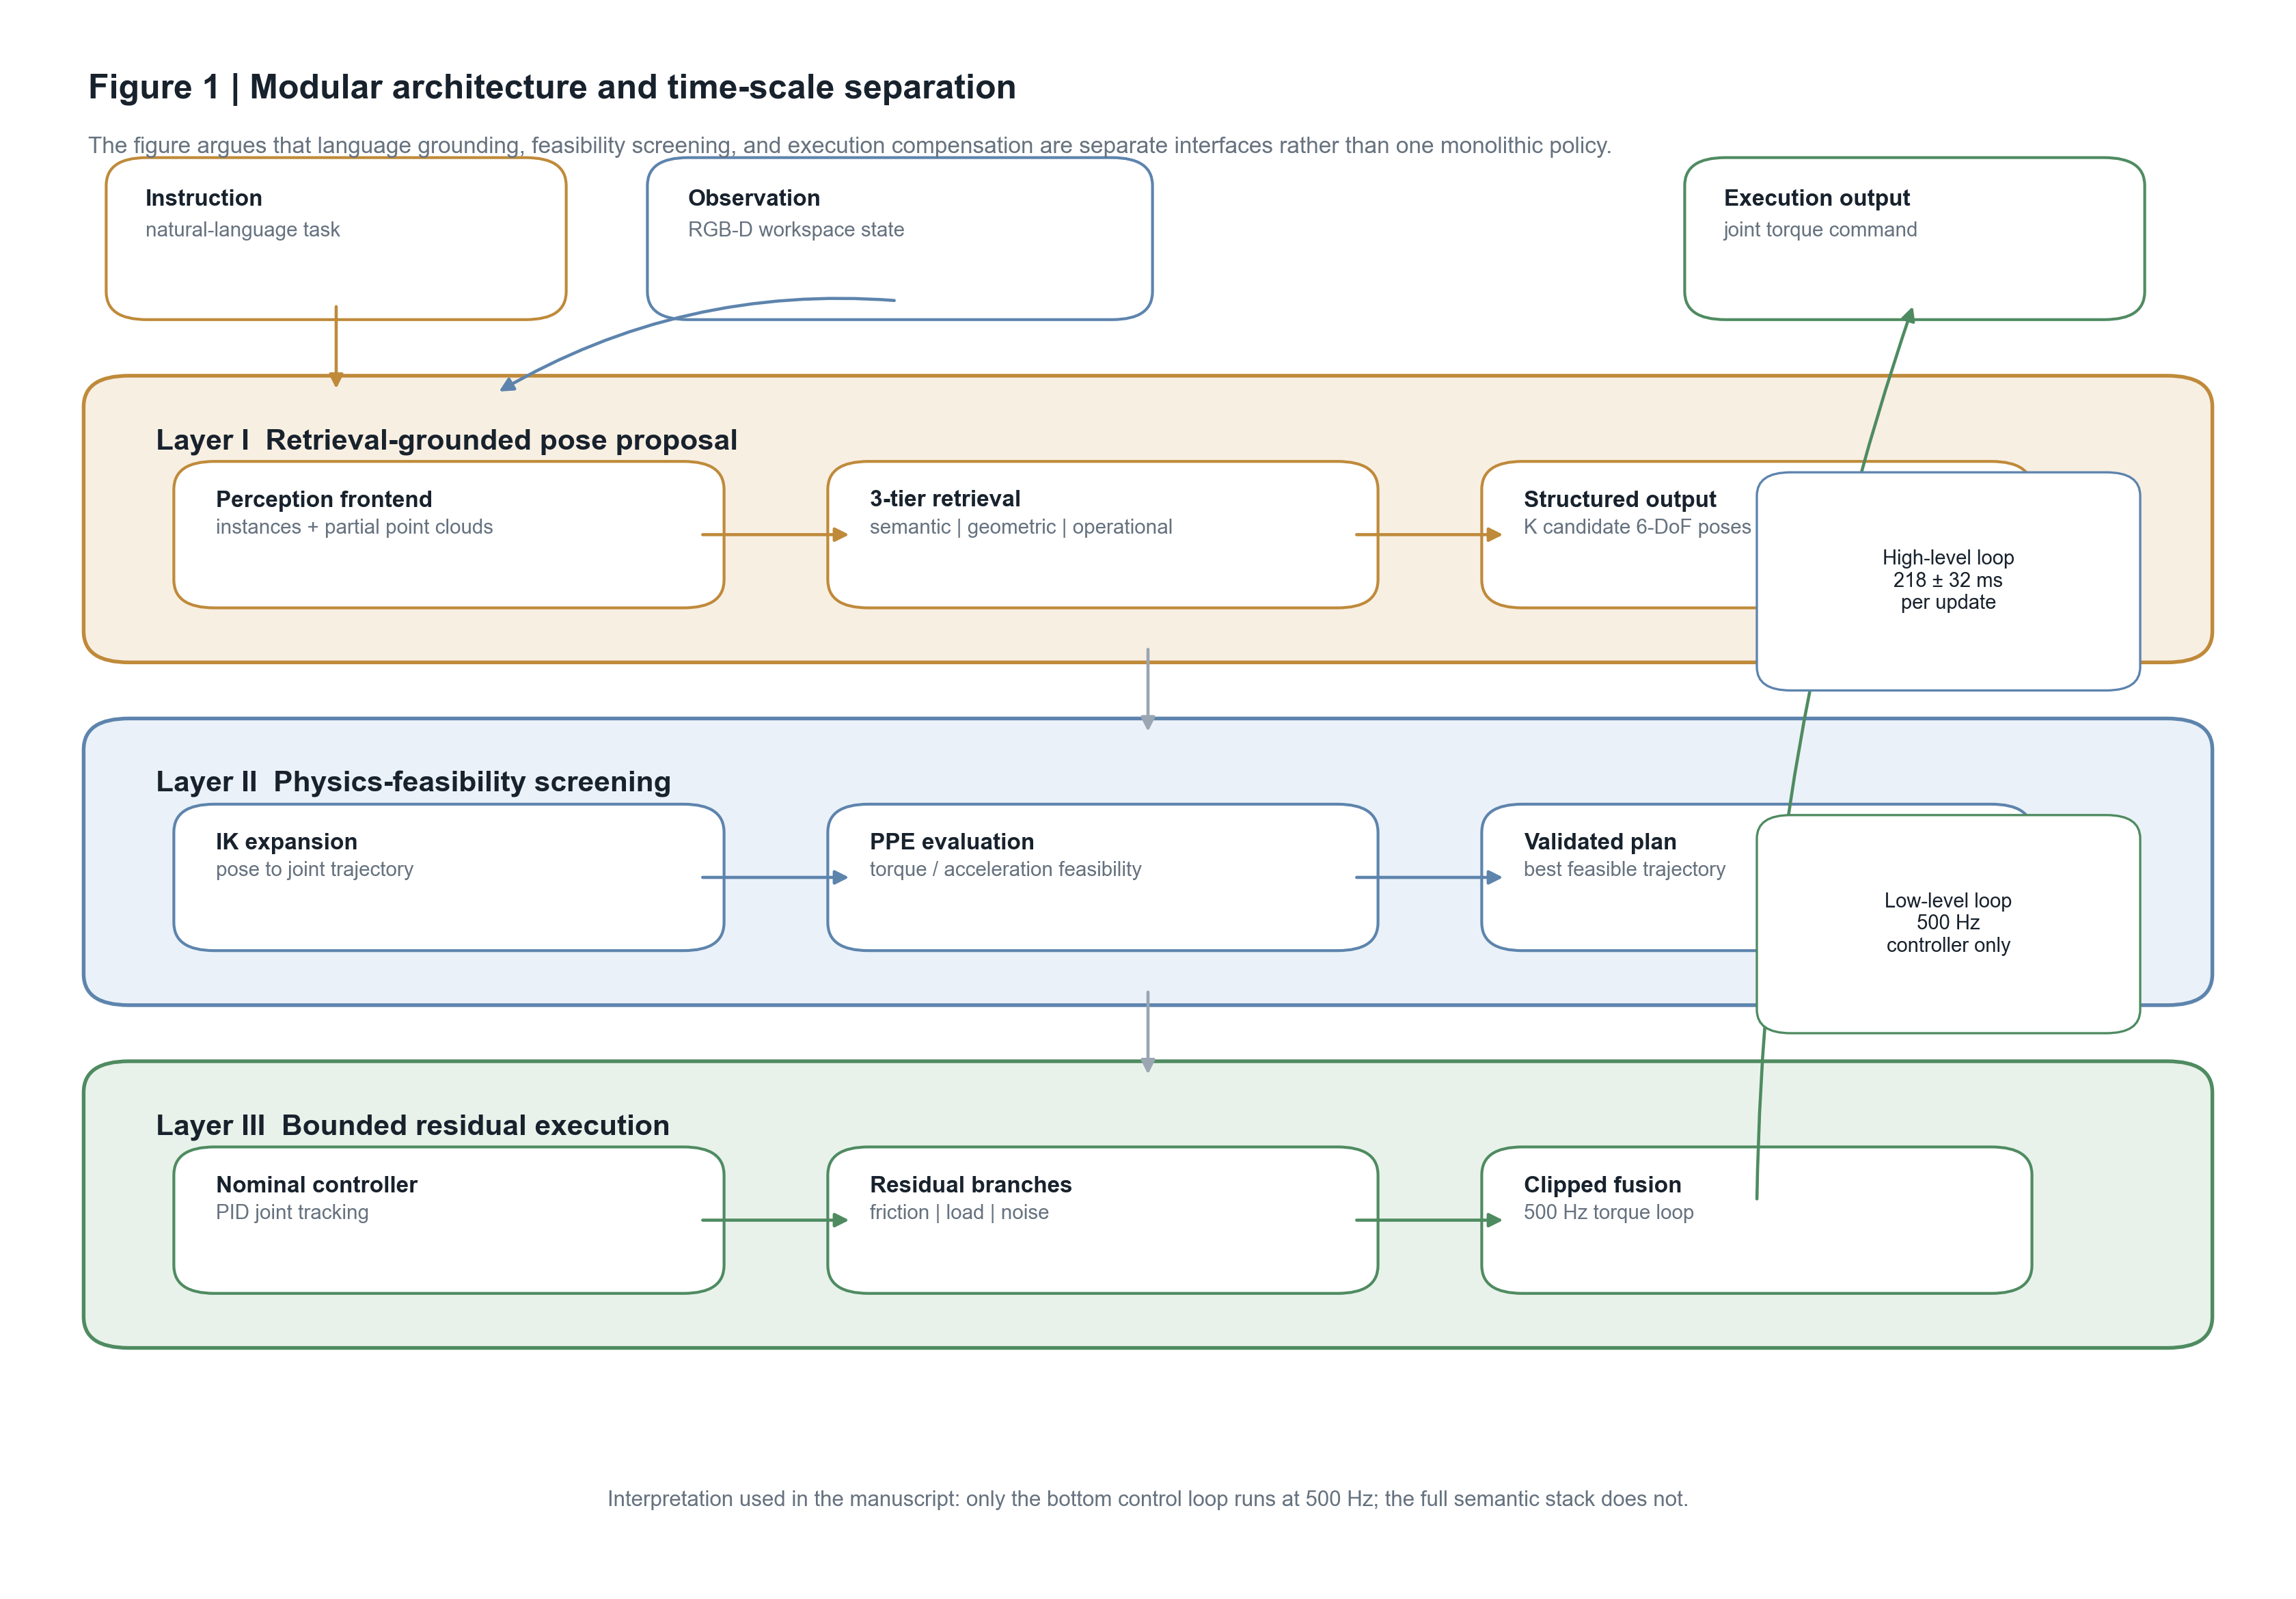
\includegraphics[width=\columnwidth]{fig1_architecture}
\caption{S2P2E three-layer architecture. The framework receives natural language instruction and RGB-D observation. Layer I (3D-Physics RAG) retrieves task-relevant 3D knowledge and generates 6-DoF target poses. Layer II (PPE) verifies physical feasibility and injects physics-consistency embeddings. Layer III (Hierarchical Residual Control) decomposes execution compensation into specialized sub-networks with adaptive gating and safety bounds. Output: joint torque command $\tau$.}
\label{fig:architecture}
\end{figure}

Processing: RGB-D camera captures the workspace and the user provides an instruction. Layer I segments the scene, retrieves knowledge entries, and uses retrieval-conditioned decoding to produce candidate 6-DoF target poses $\{T_1, \ldots, T_K\}$. Layer II computes a joint-space trajectory via IK and evaluates it with PPE. Layer III tracks the validated trajectory with PID plus clipped residual compensation. We distinguish two time scales throughout the paper: the high-level semantic-planning loop, which takes $218\pm32$~ms per update ($N=500$ measurements), and the low-level torque loop, which runs at 500~Hz.

% =========================== 4. LAYER I ===========================
\section{Layer I: 3D-Physics RAG}

\subsection{Three-Tier Physical Knowledge Base}

\textbf{Semantic Tier:} Category label, functional tags, and natural-language affordance description. Encoded via a text encoder aligned with the pose generator vocabulary.

\textbf{Geometric Tier:} 3D scene representation annotated with local affordance cues such as surface curvature, normal direction, and approachability. This tier provides the information most directly related to visibility, collision risk, and approach direction.

\textbf{Operational Tier:} For each $(\text{object}, \text{task})$ pair, we store 6-DoF grasp pose candidates, quality scores, and task-specific constraints. Encoded as structured vectors projected into a shared $d=512$ embedding space.

Three-tier embeddings are concatenated and indexed in FAISS (IndexFlatIP, exact inner-product search). The reported manipulation benchmark uses a 12,000-entry experiment-facing working index sampled from the broader S2P2E-RAG release, enabling sub-millisecond retrieval while keeping online ablations fixed across methods.

\subsection{Perception Frontend and Retrieval}

RGB-D observation $\rightarrow$ SAM~2~\cite{ravi2024sam2} instance segmentation + DepthAnything V2~\cite{yang2024depthanythingv2} depth estimation $\rightarrow$ partial point clouds $\rightarrow$ point-cloud feature extraction via PointNeXt architecture $\rightarrow$ scene query embedding $\mathbf{s} \in \mathbb{R}^{512}$. A frozen language model parses the instruction into target object(s), task type, and textual constraints. We use the inferred task type to select retrieval weights $\mathbf{w} = [w_{\mathrm{sem}}, w_{\mathrm{geo}}, w_{\mathrm{op}}]$ from a small predefined set (\emph{pick}, \emph{place}, \emph{insert}, \emph{pour}, \emph{tool-use}), rather than learning these weights end-to-end. In the reported experiments, this task-to-weight mapping is a fixed rule-based preset table, and the language-model backbone is kept frozen across all Layer~I ablations.

Retrieval uses
\[
\mathrm{score}(\mathbf{k}, \mathbf{s}, \mathbf{w}) =
\sum_{\mathrm{tier}} w_{\mathrm{tier}} \cdot
\cos(\mathbf{e}_{\mathrm{tier}}(\mathbf{k}), \mathbf{s}).
\]
Top-$K$ entries ($K=5$) are retrieved. Sensitivity analysis shows $K\in[3,10]$ yields $<3\%$ GSR variation.

\subsection{Cross-Attention Fusion and Pose Generation}

Retrieved embeddings $\{\mathbf{k}_j\}$ are passed to a cross-attention block, with the scene query $\mathbf{s}$ as the query. The resulting retrieval context is appended to the frozen model's instruction tokens, and the decoder emits $K$ pose candidates in the structured format $(x,y,z,q_w,q_x,q_y,q_z,g)$, where $g$ denotes gripper state. Greedy decoding is used throughout the manipulation experiments. Decoding is followed by deterministic post-processing: quaternion normalization, workspace-bound checks, and IK validation. If a generated pose fails any of these checks, the next candidate is evaluated.

\begin{figure}[t]
\centering
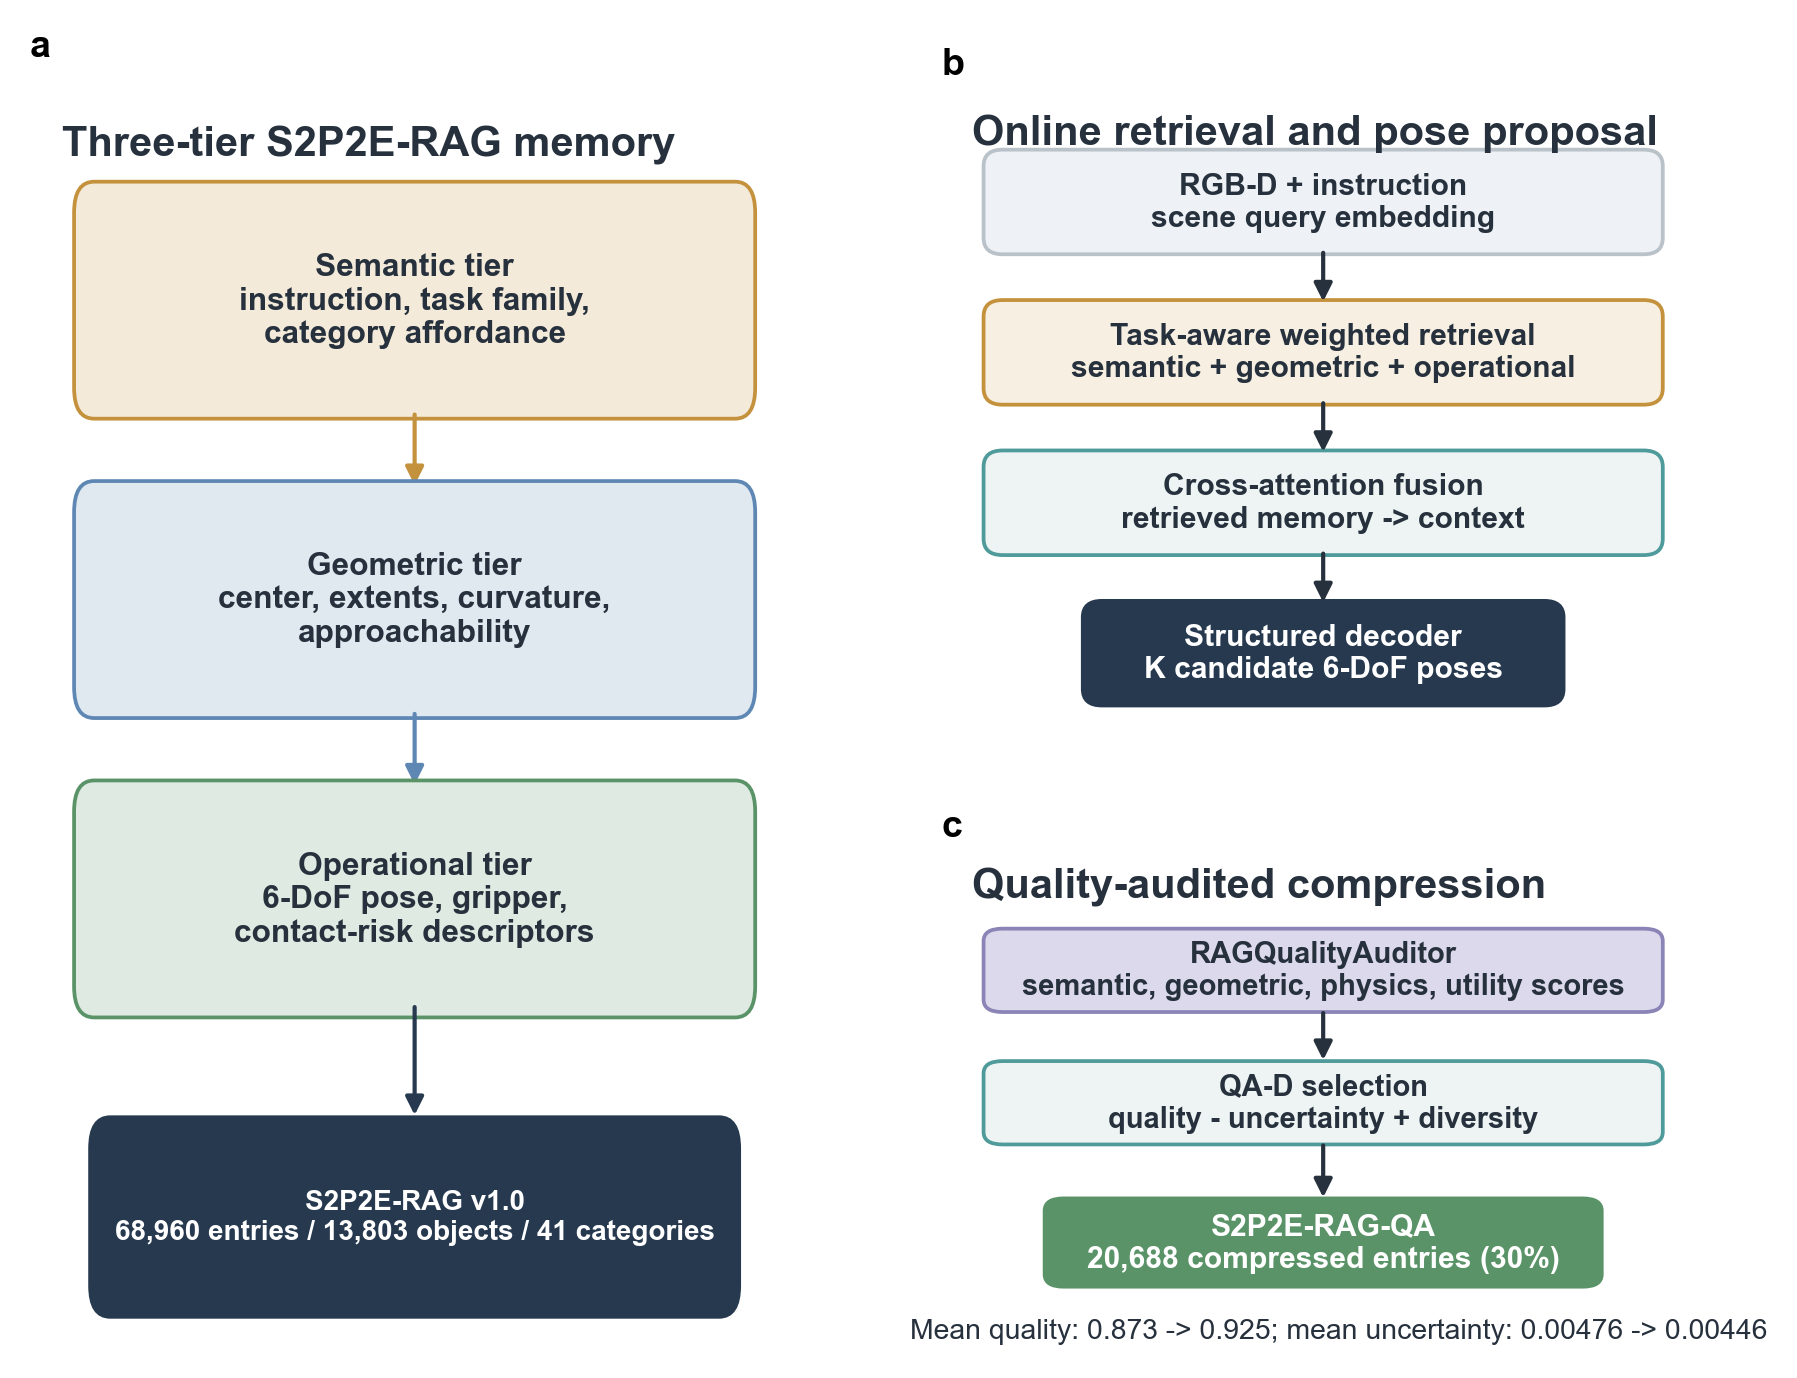
\includegraphics[width=\textwidth]{fig2_knowledge_base.png}
\caption{Three-tier knowledge base structure and retrieval pipeline. Left: automated construction of semantic, geometric, and operational entries from public assets, simulation, and grasp-pose proposals. Middle: quality-audited compression with the RAGQualityAuditor used to select a compact S2P2E-RAG-QA subset. Right: online retrieval from perception to weighted retrieval and structured pose generation.}
\label{fig:knowledge_base}
\end{figure}

\subsection{Automated Knowledge Base Construction}

3D models are sourced from Objaverse and ShapeNet, then normalized into a retrieval schema that separates semantic, geometric, and operational evidence. The public S2P2E-RAG v1.0 release contains 68,960 structured entries derived from 13,803 objects across 41 object categories and five task families. Each entry records task-conditioned semantic labels, geometry summaries, approach-direction descriptors, grasp-pose proposals, physics proxy fields, quality flags, and provenance identifiers so that retrieval behaviour can be audited entry by entry rather than treated as an opaque embedding cache.

To make the released retrieval memory smaller and more defensible, we train a RAGQualityAuditor over the generated entries. The auditor predicts semantic validity, geometric-action consistency, physics feasibility, retrieval utility, and overall quality, with Monte-Carlo dropout used as an uncertainty proxy. We then form S2P2E-RAG-QA by quality-audited diverse selection (QA-D), retaining 20,688 entries at the 30\% compression point. In the source-data benchmark, QA-D increases mean quality from 0.873 in the full generated pool to 0.925 at 30\% retention and lowers uncertainty from 0.00476 to 0.00446 (Fig.~\ref{fig:rag_quality}). Human audit ranges archived in the source data further indicate that QA-D raises the manual accept rate from 39.0--45.0\% in the full generated pool to 92.0--96.0\% in the compressed subset, while reducing the manual reject rate from 7.0--11.0\% to 0.0--1.0\%. The pose-memory proxy is reported as a comparability check rather than an optimization claim: the compact audited set preserves the retrieval interface while prioritizing entry quality, calibration, and release auditability.

% =========================== 5. LAYER II ===========================
\section{Layer II: Physics Prior Encoder}

\subsection{Motivation}

Language-conditioned pose generators are driven primarily by statistical regularities rather than equation-of-motion solutions. A geometrically plausible pose may still correspond to torques outside actuator limits or trajectories near singular configurations. PPE embeds an inverse-dynamics prior into policy learning.

\subsection{Stage 1: Inverse Dynamics Pretraining}

$10^6$ motion trajectories are generated in MuJoCo by sampling Franka Panda's 7-DoF workspace. Each sample contains $(q, \dot{q}, \ddot{q}, \tau)$, with $\tau$ computed by the recursive Newton-Euler algorithm under the simulator's rigid-body model. PPE is an MLP with four hidden layers of width 512 and embodiment-conditioned feature modulation receiving embodiment parameters $\mathbf{c} = [L_1\ldots L_7, m_1\ldots m_7, I_1\ldots I_7]$. This conditioning scheme enables a single PPE to be adapted across embodiments without retraining from scratch.

Pretraining objective:
\[
\mathcal{L}_{\mathrm{ID}} =
\mathrm{MSE}(\hat{\tau}, \tau) +
\lambda_{\mathrm{physics}} \cdot
\mathcal{L}_{\mathrm{consistency}}.
\]
$\mathcal{L}_{\mathrm{consistency}}$ is implemented as a conservative regularizer on actuator-bound slack and temporal torque smoothness, rather than as an energy-conservation penalty. This choice avoids imposing conservative-system assumptions that do not generally hold under actuation, friction, and contact. $\lambda_{\mathrm{physics}} = 0.1$ by grid search. After pretraining, PPE achieves inverse-dynamics RMSE of $0.047$~N$\cdot$m on held-out trajectories.

\subsection{Stage 2: Injection into Policy Networks}

The frozen PPE is integrated into actor-critic networks through three mechanisms:

\textbf{(a) Physics Feature Injection:} PPE penultimate-layer activations are concatenated with policy observation encodings in both Actor and Critic.

\textbf{(b) Reward Shaping:} For each actor-proposed action, PPE predicts torques and applies a penalty when predicted torques exceed hardware limits:
\[
r_{\mathrm{shaped}} =
r_{\mathrm{task}} -
\lambda_{\mathrm{viol}} \cdot
\max(0, |\hat{\tau}| - \tau_{\max}),
\]
with $\lambda_{\mathrm{viol}} = 0.5$.

\textbf{(c) Contrastive Physics Embedding:} Positive pairs are feasible actions and negative pairs are perturbed infeasible actions:
\[
\mathcal{L}_{\mathrm{contrast}} =
-\log
\left[
\frac{\exp(\mathrm{sim}(z^+)/T)}
{\sum \exp(\mathrm{sim}(z)/T)}
\right], \quad T = 0.1.
\]

\subsection{Cross-Embodiment Generalization}

Embodiment-conditioned modulation enables transfer: PPE achieves $0.072$~N$\cdot$m RMSE on KUKA iiwa (vs.\ $0.047$~N$\cdot$m native) and $0.089$~N$\cdot$m on UR5e, corresponding to 53\% and 47\% error reductions relative to unconditioned transfer. Figure~\ref{fig:ppe}(b) is included as supporting evidence that the pretrained prior itself remains portable across robot embodiments at the inverse-dynamics level. We stress that this section evaluates inverse-dynamics transfer only; downstream manipulation transfer across embodiments is outside the validated claim scope of the present study.

To make the physical assumptions more explicit, Fig.~\ref{fig:mechanical_model} summarizes the rigid-body abstraction used throughout Layers~II and III. The figure highlights the kinematic chain, end-effector transform, representative link-length parameters, contact force, gravity load, and residual torque injection. We do not claim that this drawing is a complete dynamic derivation of the manipulator. Its purpose is narrower: to make clear which physical quantities are explicitly modeled by PPE and which disturbances are left to the bounded residual controller at execution time.


\begin{figure}[t]
\centering
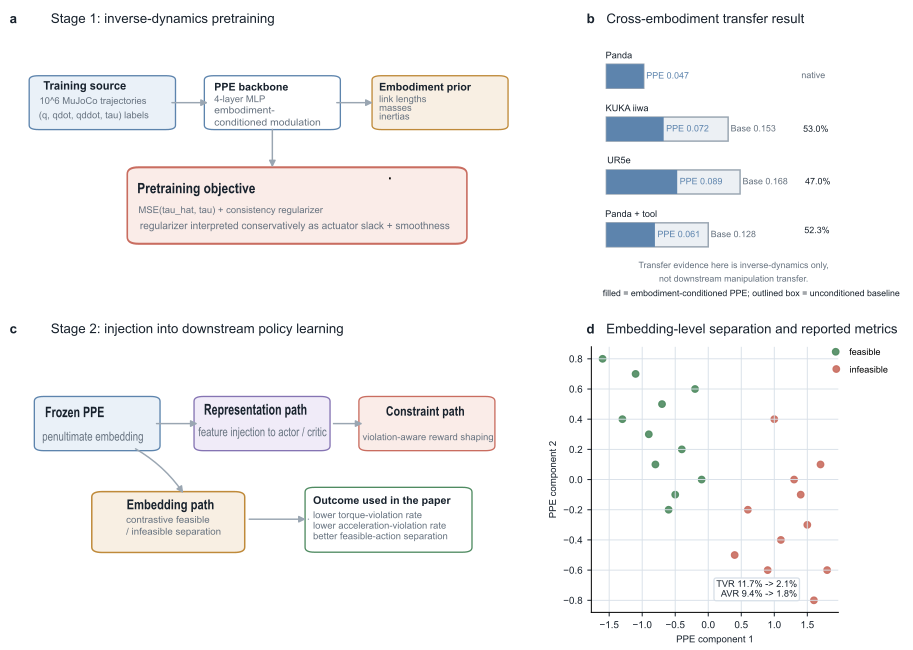
\includegraphics[width=\textwidth]{fig3_ppe}
\caption{Physics Prior Encoder two-stage training. (a) Supervised inverse-dynamics pretraining with embodiment-conditioned modulation and conservative consistency regularization. (b) Injection into actor-critic networks through feature injection, reward shaping, and contrastive separation of feasible versus infeasible actions. (c) Embedding-level separation and outcome metrics.}
\label{fig:ppe}
\end{figure}

\begin{figure}[t]
\centering
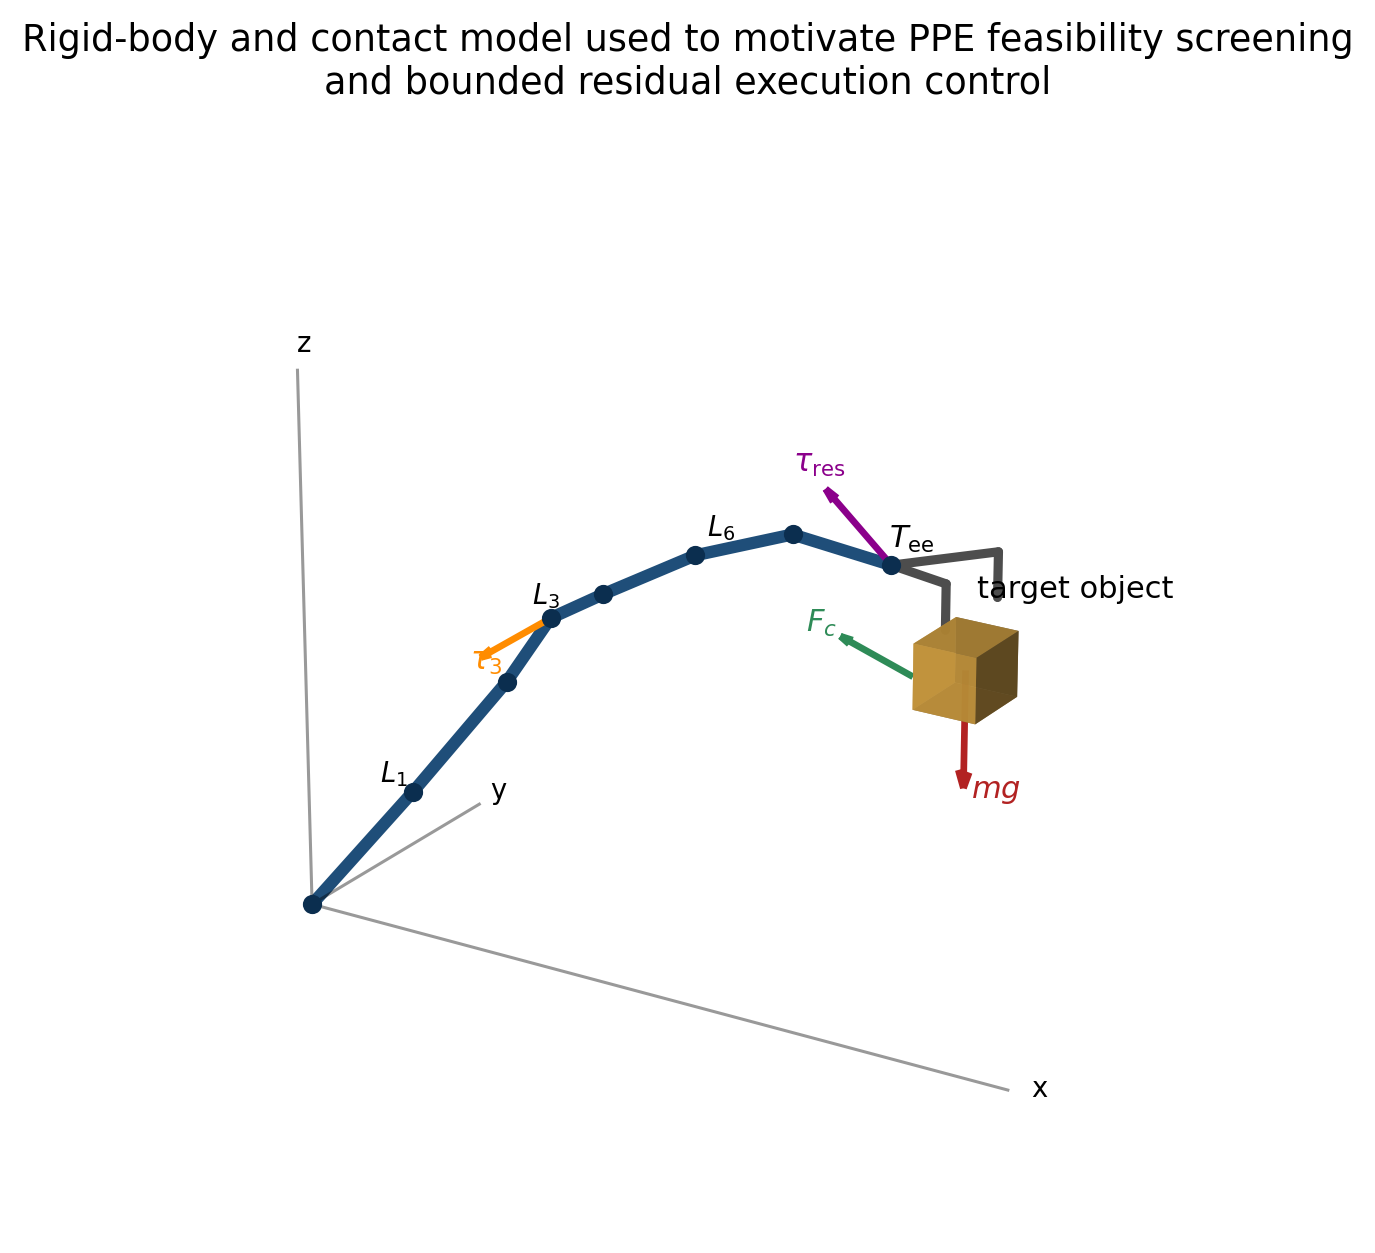
\includegraphics[width=\columnwidth]{fig8_mechanical_model}
\caption{Mechanical-perspective physical model used to bridge feasibility screening and residual control. The schematic makes explicit the rigid-body chain, end-effector transform $T_{\mathrm{ee}}$, representative link lengths $L_i$, gravity load $mg$, contact force $F_c$, and residual torque injection $\tau_{\mathrm{res}}$. In the manuscript's interpretation, PPE is responsible for screening trajectories against the structured part of this model, whereas Layer~III compensates for the residual mismatch that remains at contact time.}
\label{fig:mechanical_model}
\end{figure}

% =========================== 6. LAYER III ===========================
\section{Layer III: Hierarchical Residual Control}

\subsection{Problem Formulation}

Layer III receives validated joint-space reference trajectories $q_{\mathrm{ref}}(t)$ from Layer II. PID nominal torques are
\[
\tau_{\mathrm{PID}}(t) =
K_p e(t) +
K_i \int e(t)\,dt +
K_d \dot{e}(t),
\]
with $e(t) = q_{\mathrm{ref}}(t) - q(t)$. The executed command is
\[
\tau(t) =
\tau_{\mathrm{PID}}(t) + \alpha \cdot \Delta\tau(t),
\]
where $\alpha \in [0,1]$ and $|\Delta\tau| \leq 0.2 |\tau_{\mathrm{PID}}|$ after clipping.

\subsection{Specialized Residual Sub-Networks}

\textbf{FrictionNet:} A temporal convolutional network receiving $(\dot{q}, \tau_{\mathrm{history}})$ and predicting $\hat{\tau}_{\mathrm{fric}}$.

\textbf{LoadNet:} A 3-layer MLP receiving wrist force-torque $F_{\mathrm{sensor}}$ and current pose $T_{\mathrm{cur}}$, predicting $\hat{\tau}_{\mathrm{load}}$.

\textbf{NoiseNet:} A temporal filter receiving a short history of end-effector pose estimates and predicting $\hat{\tau}_{\mathrm{noise}}$.

The total residual is
\[
\Delta\tau =
\hat{\tau}_{\mathrm{fric}} +
\hat{\tau}_{\mathrm{load}} +
\hat{\tau}_{\mathrm{noise}}.
\]
The three modules are trained jointly and adapted online with separate learning rates.

\subsection{Task-Aware Gating Network}

GateNet is a 2-layer MLP receiving one-hot task-phase encoding (\texttt{free\_motion}, \texttt{approach}, \texttt{contact}, \texttt{transport}, \texttt{release}) and contact-force magnitude $|F_{\mathrm{sensor}}|$. It outputs $\alpha \in [0,1]$ via sigmoid. The auxiliary loss
\[
\mathcal{L}_{\mathrm{gate}} =
(\alpha_{\mathrm{free}} - 0)^2 +
(\alpha_{\mathrm{contact}} - 1)^2
\]
encourages PID dominance in free space and stronger residual contribution during contact. The task phase is provided by the commanded state machine, not by a second learned language inference module.

\subsection{Stability Considerations}

Residual correction is bounded as
\[
\Delta\tau_{\mathrm{clipped}} =
\mathrm{clamp}(\Delta\tau, -0.2|\tau_{\mathrm{PID}}|, 0.2|\tau_{\mathrm{PID}}|)
\]
Classical Lyapunov analyses for bounded additive perturbations motivate this clipping rule as a conservative controller design heuristic. In our adaptive gated setting, however, we do \emph{not} claim a full formal proof of closed-loop stability. Instead, we report the empirical observation that the controller-evaluation runs reported in this paper exhibited no torque-limit violations and no unstable oscillations under the 20\% clip.

\begin{figure}[t]
\centering
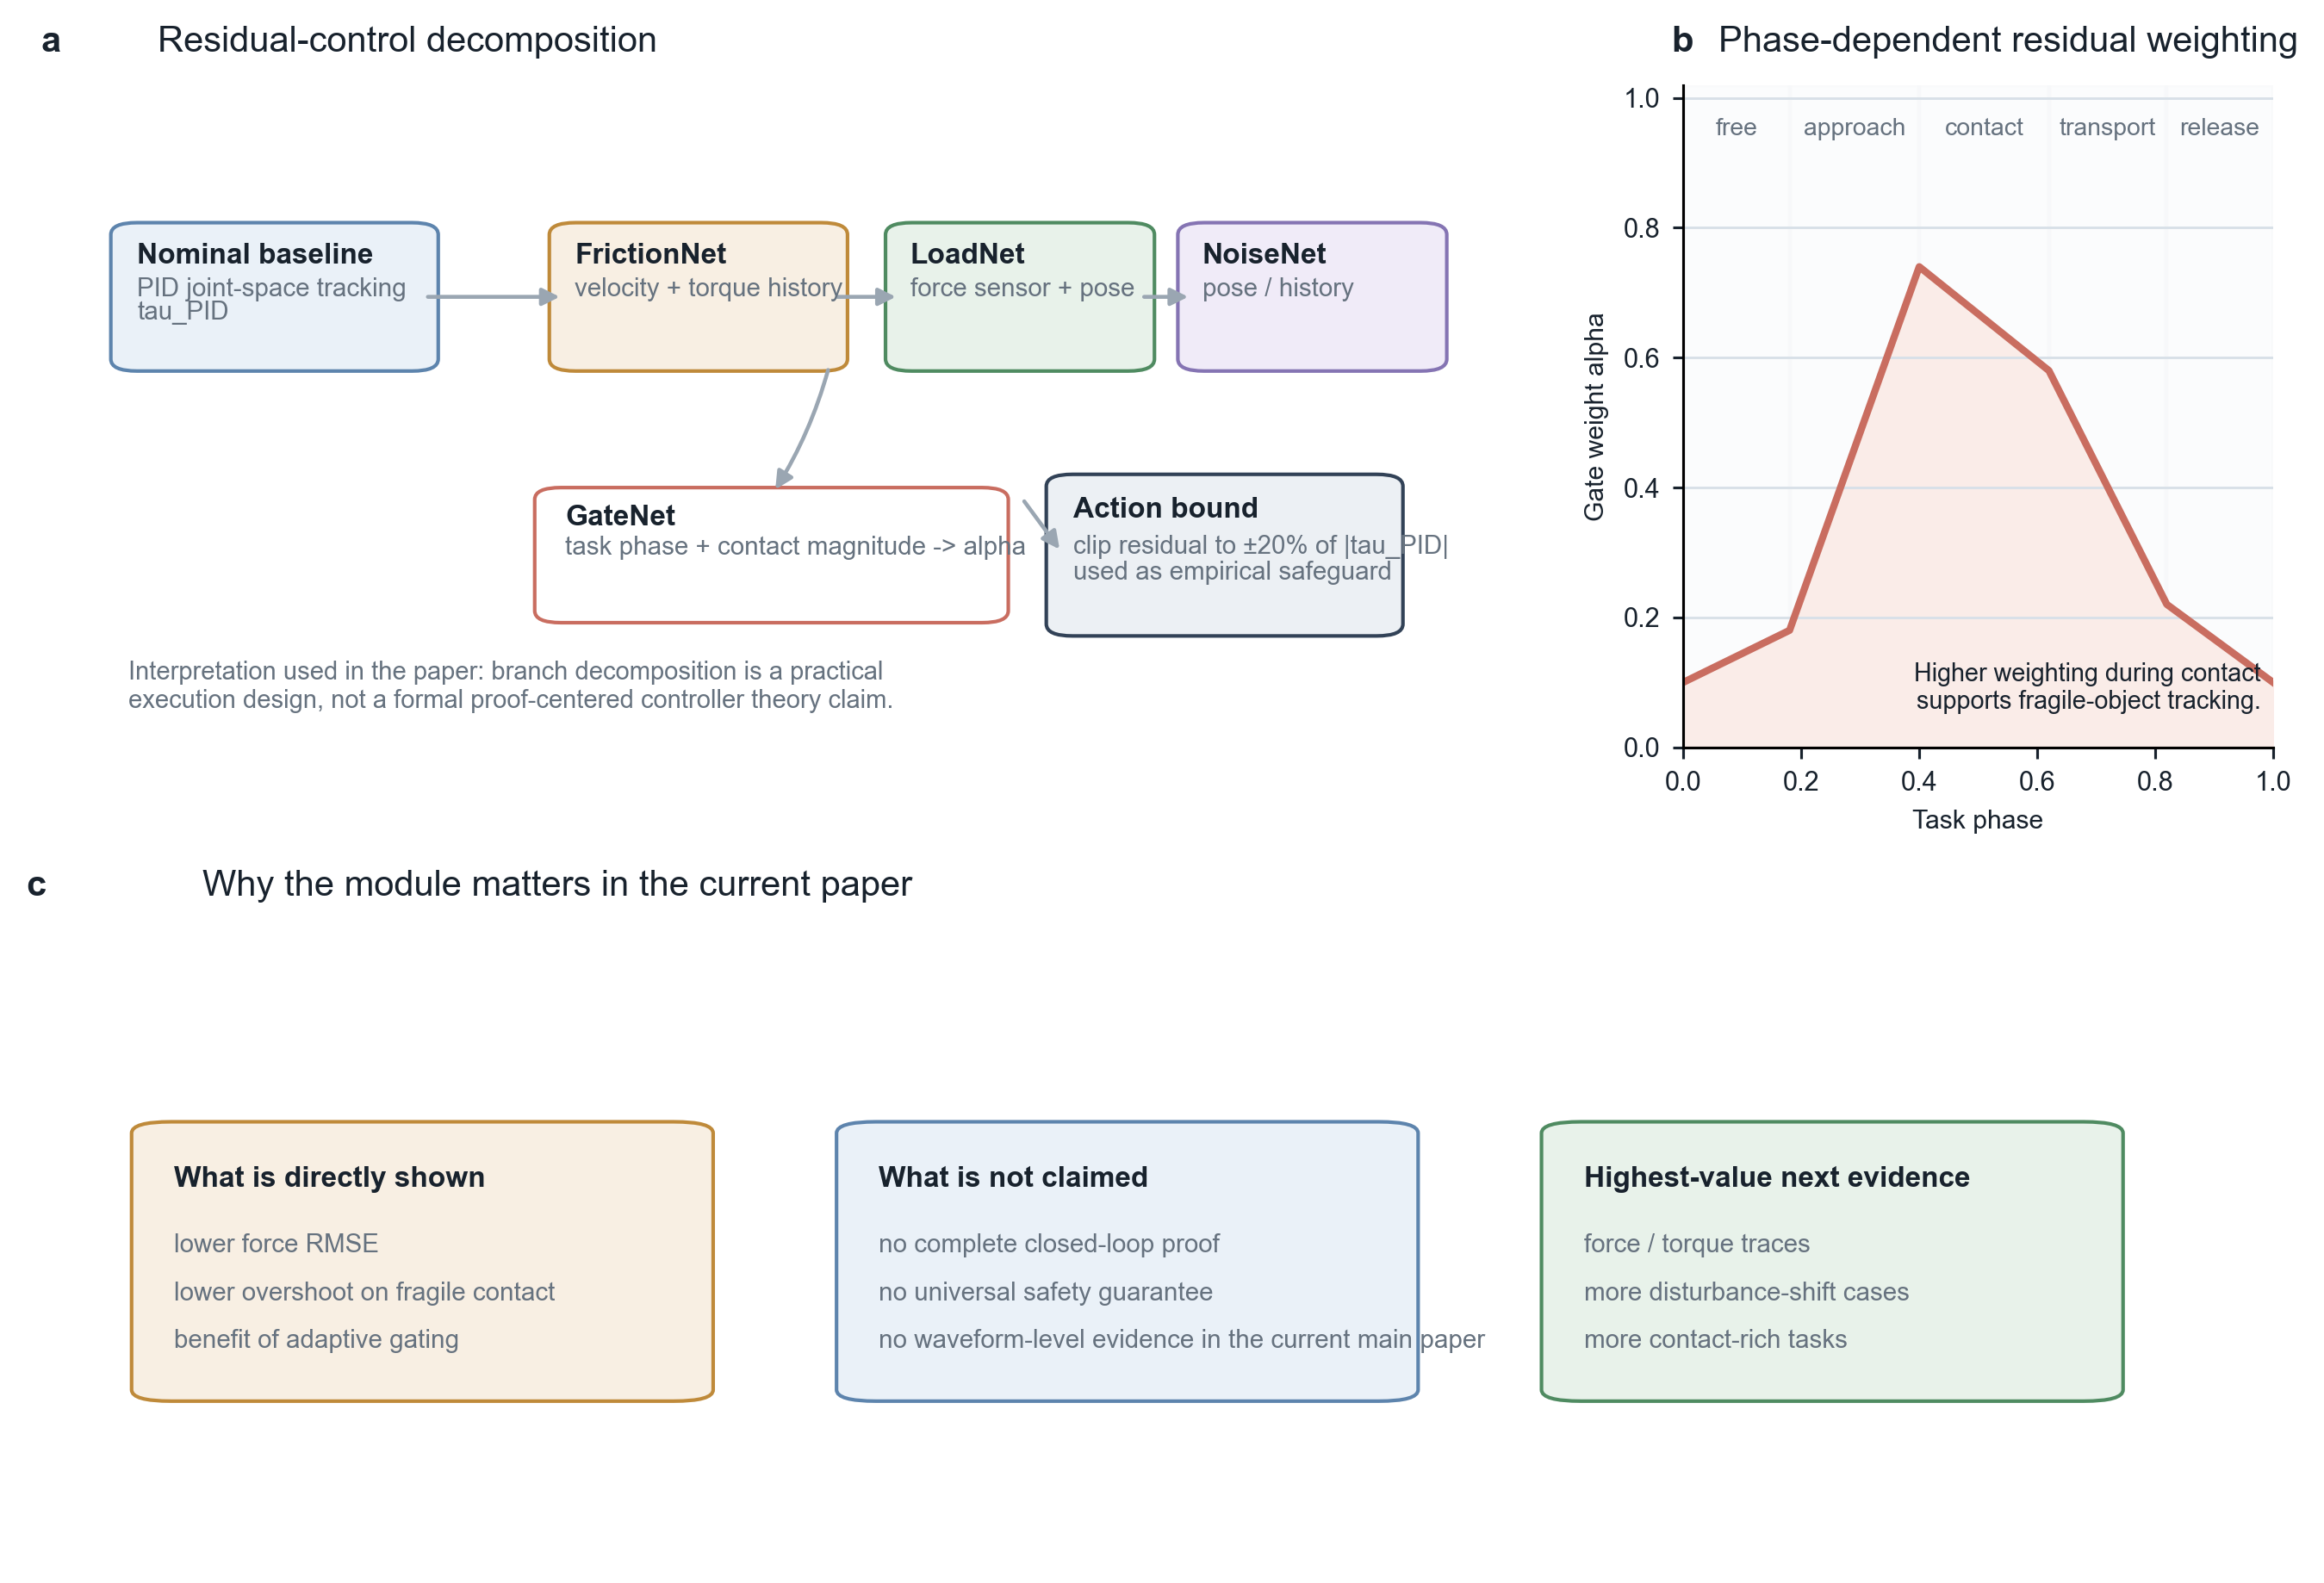
\includegraphics[width=\linewidth]{fig4_residual_control}
\caption{Hierarchical residual control architecture. Classical PID provides nominal torque. FrictionNet, LoadNet, and NoiseNet compensate distinct disturbance sources. GateNet outputs the adaptive residual weight $\alpha$, and the action-bounding layer clips residual magnitude before torque execution. The task-phase strip summarizes how the controller shifts between conservative free-space tracking and stronger contact-time compensation.}
\label{fig:residual_control}
\end{figure}

% =========================== 7. EXPERIMENTS ===========================
\section{Experiments}

\subsection{Experimental Setup}

\textbf{Hardware:} Franka Emika Panda 7-DoF arm, parallel-jaw gripper, Intel RealSense D435 wrist-mounted camera. \textbf{Simulation:} Isaac Sim 2024.1 and MuJoCo 2.3.7. \textbf{Knowledge base:} a 12,000-entry experiment-facing working index sampled from the 68,960-entry S2P2E-RAG release. Unless otherwise stated, each method is evaluated on the same 50-scene library and the same object placements for each seed. Main performance tables report mean $\pm$ SD across five random seeds; source-data files additionally record the total number of executed episodes or trajectories supporting each row. For significance testing, we form matched per-scene outcome vectors under identical scene instances and object placements, apply paired comparisons to those matched scene-level outcomes, and use Bonferroni correction across reported pairwise tests. Additional implementation details, module settings, and claim-boundary notes are summarized in the supplementary materials.

\textbf{Baselines:} (a) OpenVLA-7B~\cite{kim2024openvla}; (b) ManipLLM~\cite{li2024manipllm}; (c) GPT-4V + chain-of-thought (reported as a protocol-controlled reference rather than a central reproducible baseline); (d) PID-only with AnyGrasp~\cite{fang2024anygrasp}; (e) TD-MPC2~\cite{hansen2024tdmpc2}; (f) OpenVLA + our retrieval module; and (g) S2P2E ablated variants. These baselines span general VLA policies, modular grasping stacks, and end-to-end control, so they should be interpreted as complementary reference points rather than perfectly matched apples-to-apples competitors. Our main causality claims therefore rely most heavily on the matched internal comparisons (`w/o RAG', `w/o PPE', `w/o Residual') and on the OpenVLA+KB comparison, which isolates the contribution of the retrieval layer under a shared high-level backbone.

\textbf{Training protocol used for the reproduced stack:} Layer~I uses embedding dimension $d=512$, retrieval top-$K=5$, and loss weights $\lambda_{\mathrm{pose}}=5.0$, $\lambda_{\mathrm{gripper}}=1.0$, and $\lambda_{\mathrm{retrieval}}=0.2$. Layer~II uses a 4-layer PPE with hidden dimension 512, $\lambda_{\mathrm{physics}}=0.1$, and trajectory length 24. Layer~III uses residual history length 8, clip ratio 0.2, and $\lambda_{\mathrm{gate}}=0.5$. A secondary policy-bridge sanity check uses 1,134 converted DROID transitions~\cite{khazatsky2024droid} to test whether the feasibility-conditioned action interface can be optimized on externally sourced robot data; it is not used as primary benchmark evidence. We report these settings explicitly so that the training recipe can be reproduced rather than inferred from aggregate benchmark results alone.

\textbf{Dataset splits, leakage prevention, and bias:} The reported reproduction uses fixed train/validation/test partitions at the scene-instance level, with task-family balancing across splits and a held-out set of 20 unseen objects for the clutter benchmark. For sim-to-real evaluation, the 10 hardware-deployable tasks are selected as a strict deployment subset and are not reused for model selection. The embodiment-transfer results use held-out trajectories that are separated by embodiment identity rather than by random frame sampling alone. We emphasize these details because robotics pipelines are unusually vulnerable to leakage through repeated scene layouts, near-duplicate object instances, temporally adjacent trajectories, or simulator-specific artifacts. The present dataset mix is also biased toward rigid and semi-rigid tabletop objects, synthetic rigid-body dynamics, and front-facing manipulation viewpoints, so the reported conclusions should not be extrapolated to deformable manipulation, heavy occlusion, or highly dynamic mobile interaction without additional validation.

\textbf{Evidence hierarchy and generalization axes:} To avoid over-compressing distinct claims into a single notion of ``generalization'', we treat the empirical evidence in four layers. First, module-level validation asks whether each interface in the stack behaves as intended under controlled optimization conditions. Second, the matched clutter benchmark tests primary task performance under shared scene instances. Third, targeted physical evaluations probe whether the claimed mechanism of improvement is consistent with reduced violations and better contact behavior. Fourth, transfer-oriented experiments assess progressively broader generalization axes: across task families, across held-out objects, across embodiments at the inverse-dynamics level, and from simulation to bounded hardware deployment under perturbation stress tests. These axes support the bounded tabletop claims reported here; they should not be read as evidence of unrestricted open-world or cross-robot deployment.

\textbf{Main text versus supplementary scope:} We use the main paper to report the minimal evidence needed to support the central systems claim, namely that retrieval grounding, feasibility filtering, and bounded residual control make complementary contributions under matched manipulation conditions. Supporting materials are separated into an explicit supplementary package so that reproducibility-critical implementation details do not remain implicit. The submission package is organized as \texttt{Supplementary\_Information.tex} together with machine-readable files under \texttt{source\_data/}; it contains leakage-prevention rules, table-level sample definitions, checkpoint-selection rules, value-provenance records, and source-data exports.

\subsection{Module-Level Quantitative Verification}

\begin{table}[!htbp]
\centering
\caption{Module-level validation metrics for the reproduced S2P2E stack. Metrics are taken from the best checkpoints of the reported reproduction pipeline.}
\label{tab:module_metrics}
\small\setlength{\tabcolsep}{5pt}
\resizebox{\textwidth}{!}{%
\begin{tabular}{@{}l c c c c@{}}
\toprule
Module & Best epoch & Primary validation metric & Secondary metric 1 & Secondary metric 2 \\
\midrule
Layer~I (3D-Physics RAG) & 2 & Pose MAE $=0.0244$ & Pose loss $=0.00138$ & Retrieval loss $=2.0457$ \\
Layer~II (PPE) & 3 & RMSE $=0.0406$ & MSE $=0.00165$ & Consistency $=7.97\times10^{-4}$ \\
Layer~III (Residual control) & 4 & Residual loss $=0.00145$ & Gate loss $=0.0723$ & Command norm $=2.7321$ \\
Joint stack & 4 & Joint val.\ loss $=0.0492$ & Pose loss $=0.0131$ & Tau loss $=0.00985$ \\
Policy bridge (DROID subset) & 2 & Critic loss $=1.80\times10^{-7}$ & Actor loss $=-0.0392$ & Contrastive loss $=0.6851$ \\
\bottomrule
\end{tabular}
}
\end{table}

Table~\ref{tab:module_metrics} serves a different role from the task-level tables that follow. Rather than asking whether the full system succeeds on end tasks, it asks whether each interface in the stack is numerically well behaved under training. This distinction matters for a modular systems paper. A strong end-task result without module-level diagnostics would make it difficult to know whether the gains come from the intended mechanism or from compensating errors elsewhere in the stack. Conversely, the low Layer~II RMSE, low Layer~III residual loss, and stable joint losses suggest that the final policy is not being carried by a single unstable component.

\begin{table}[!htbp]
\centering
\caption{Dataset and evaluation accounting. Counts refer to the locked protocol used for the reported manuscript results.}
\label{tab:dataset_accounting}
\small\setlength{\tabcolsep}{4pt}
\resizebox{\textwidth}{!}{%
\begin{tabular}{@{}l c c c c@{}}
\toprule
Component & Train unit & Validation/Test unit & Training or protocol count & Evaluation support \\
\midrule
Synthetic inverse dynamics & trajectory & held-out trajectory & $10^6$ / $10^4$ & $10^6$ / $10^4$ \\
Clutter benchmark & scene instance & scene instance & 50 scenes, 500 trials & 50 scenes, 500 trials \\
Unseen-object subset & object-scene pair & object-scene pair & 20 held-out objects & 120 episodes \\
Dense-clutter subset & scene instance & scene instance & $\geq10$ objects & 150 episodes \\
Hardware transfer subset & hardware episode & hardware episode & 50 episodes/method & 90 episodes/method \\
Stress-test transfer subset & hardware episode & hardware episode & 3 conditions & 30 episodes/condition \\
Policy bridge external data & transition & transition & 1,134 transitions & 1,134 + held-out 300 \\
\bottomrule
\end{tabular}
}
\end{table}

Table~\ref{tab:dataset_accounting} makes the evaluation units explicit, separating primary evidence from robustness slices. In practical terms, the paper is strongest when the reader can see which claims are anchored by matched evaluations and which claims are supported by secondary stress-test or transfer analyses.

\subsection{Grasp Success in Cluttered Environments}

We evaluate 50 cluttered tabletop scenes containing 5--15 objects with varying occlusion. Twenty objects are unseen during training. For each seed, all compared methods are executed on the same ordered scene list and the same object placements.

\begin{table}[!htbp]
\centering
\caption{Grasping performance across 50 cluttered scenes (mean $\pm$ SD, $N=5$ seeds, identical scene library per method).}
\label{tab:grasp}
\small\setlength{\tabcolsep}{5pt}
\begin{tabular}{@{}l c c c@{}}
\toprule
Method & GSR (\%) & PIR (\%) & TCR (\%) \\
\midrule
\textbf{S2P2E (full)} & $\mathbf{87.3 \pm 3.1}$ & $8.2 \pm 1.4$ & $81.6 \pm 2.9$ \\
S2P2E w/o RAG & $64.5 \pm 5.2$ & $27.1 \pm 3.8$ & $55.3 \pm 4.1$ \\
S2P2E w/o PPE & $78.9 \pm 3.7$ & $14.6 \pm 2.3$ & $71.2 \pm 3.3$ \\
S2P2E w/o Residual & $76.1 \pm 4.0$ & $11.3 \pm 1.9$ & $68.9 \pm 3.6$ \\
OpenVLA~\cite{kim2024openvla} & $58.1 \pm 4.8^{**}$ & $34.7 \pm 4.2^{**}$ & $42.5 \pm 5.1^{**}$ \\
OpenVLA + our KB & $71.3 \pm 3.5^{*}$ & $18.4 \pm 2.6^{*}$ & $63.7 \pm 2.8^{*}$ \\
ManipLLM~\cite{li2024manipllm} & $65.2 \pm 4.3$ & $28.9 \pm 3.5$ & $49.1 \pm 4.4$ \\
GPT-4V + CoT & $51.7 \pm 6.1$ & $41.2 \pm 5.8$ & $38.3 \pm 5.5$ \\
AnyGrasp + PID & $72.4 \pm 2.8$ & $9.8 \pm 1.1$ & $61.3 \pm 2.4$ \\
TD-MPC2 (end-to-end) & $53.8 \pm 6.7$ & $18.4 \pm 3.2$ & $38.7 \pm 5.9$ \\
\bottomrule
\end{tabular}
\par\smallskip\footnotesize
$^{*}\,p < 0.01$; $^{**}\,p < 0.001$ (paired comparison on matched scene instances vs.\ S2P2E full, Bonferroni corrected). GSR: Grasp Success Rate. PIR: Physical Interference Rate. TCR: Task Completion Rate.
\end{table}

S2P2E improves over both OpenVLA and OpenVLA augmented with the same retrieval memory. Relative to OpenVLA+KB, the full stack gains $+16.0$ points in GSR, lowers PIR by $10.2$ points, and improves TCR by $17.9$ points, which is consistent with the view that retrieval alone does not close the execution gap. The OpenVLA+KB row is therefore the fairest comparison for Layer I, while AnyGrasp+PID is the closest modular baseline for execution alone. We interpret Table~\ref{tab:grasp} as evidence for complementary gains from retrieval, feasibility filtering, and residual compensation, rather than as a claim that S2P2E dominates every manipulation paradigm. On the unseen-object-only subset (20 held-out objects, 120 evaluation episodes), S2P2E achieves $82.7\pm3.5\%$ GSR, $9.3\pm1.6\%$ PIR, and $76.5\pm3.2\%$ TCR, compared with $50.3\pm5.1\%$ GSR for OpenVLA and $64.8\pm4.2\%$ GSR for OpenVLA+KB. On the dense-clutter-only subset ($\geq10$ objects, 150 episodes), S2P2E records $10.4\pm1.8\%$ PIR and $84.1\pm3.7\%$ GSR, versus $38.7\pm5.2\%$ and $22.1\pm3.1\%$ PIR for OpenVLA and OpenVLA+KB respectively. These two slices map most directly to the semantic-grounding and physical-interference claims.

The ablation pattern is also mechanistically consistent with the intended design. Removing retrieval causes the largest drop in joint pose quality, which is exactly what should happen if Layer~I is carrying the burden of spatial grounding. Removing PPE leaves pose generation largely intact but weakens physical feasibility, while removing the residual path primarily affects contact robustness rather than semantic selection. This alignment between predicted function and observed degradation is important because it argues against the gains being a purely accidental consequence of extra parameters.

\subsection{Physical Constraint Violations}

\begin{figure}[t]
\centering
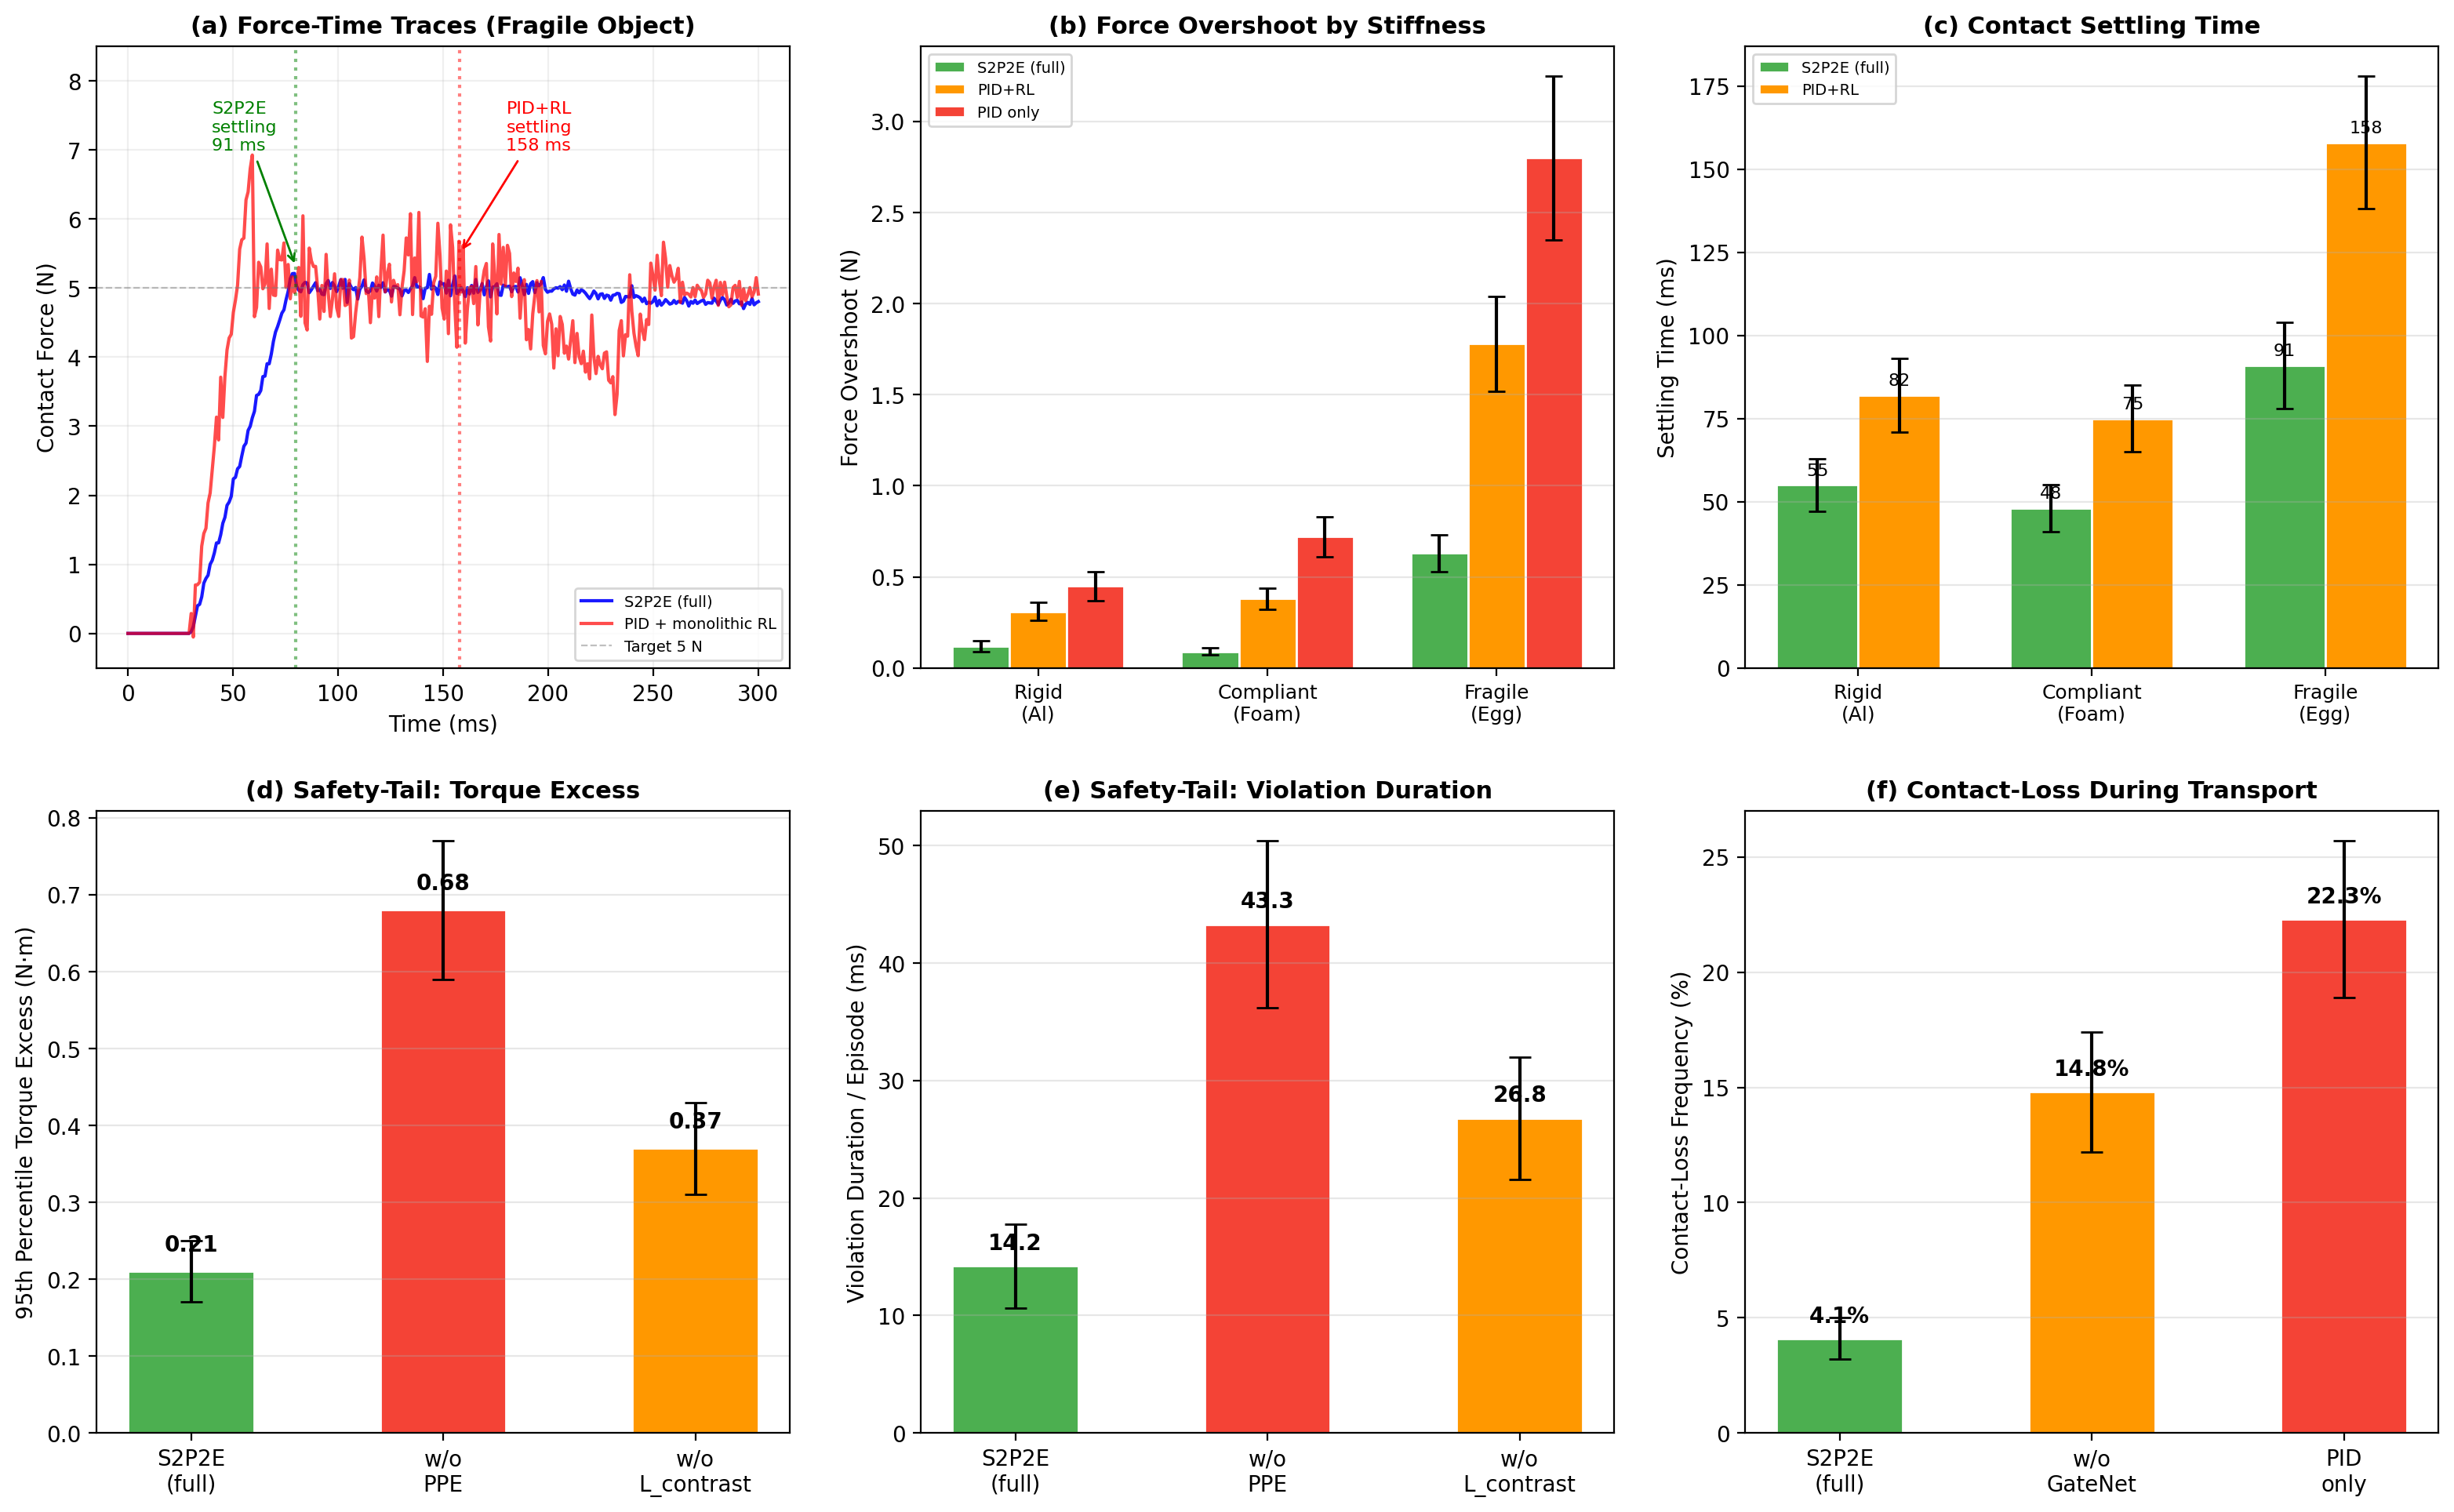
\includegraphics[width=\columnwidth]{fig10_waveform_safety.png}
\caption{Contact waveform and safety-tail evidence. (a) Representative force-time traces on fragile objects showing S2P2E settling at 91~ms versus 158~ms for PID+monolithic RL. (b) Force overshoot across stiffness regimes. (c) Settling time comparison. (d) 95th-percentile torque excess. (e) Mean violation duration per episode. (f) Contact-loss frequency during transport. All error bars are $\pm$1 SD.}
\label{fig:waveform_safety}
\end{figure}

\begin{table}[htbp]
\centering
\caption{Physical constraint violations across 500 trajectory executions (mean $\pm$ SD).}
\label{tab:violations}
\small\setlength{\tabcolsep}{3pt}
\resizebox{\columnwidth}{!}{%
\begin{tabular}{@{}l c c c@{}}
\toprule
Method & TVR (\%) & AVR (\%) & Latency (ms) \\
\midrule
\textbf{S2P2E (full)} & $\mathbf{2.1 \pm 0.4}$ & $\mathbf{1.8 \pm 0.3}$ & $218 \pm 32$ \\
S2P2E w/o PPE & $11.7 \pm 1.6$ & $9.4 \pm 1.2$ & $215 \pm 30$ \\
OpenVLA & $14.3 \pm 1.9$ & $12.6 \pm 1.7$ & $187 \pm 25$ \\
TD-MPC2 & $8.9 \pm 1.4$ & $7.2 \pm 1.1$ & $85 \pm 12$ \\
\bottomrule
\end{tabular}
}
\par\smallskip\footnotesize
\end{table}
TVR: Torque Violation Rate. AVR: Acceleration Violation Rate. The reported $218\pm32$~ms latency corresponds to one high-level semantic-planning update (perception + retrieval + pose decoding + PPE check). Only the residual torque controller runs at 500~Hz. Breakdown: SAM~2 52~ms, retrieval 11~ms, LLM 143~ms, PPE 9~ms, residual control 3~ms.

PPE reduces torque violations by 5.6$\times$ (11.7\% $\rightarrow$ 2.1\%). Importantly, this reduction is achieved with nearly unchanged planning latency (215~ms $\rightarrow$ 218~ms), so the feasibility gain is not merely a consequence of slower deliberation. Removing $\mathcal{L}_{\mathrm{contrast}}$ increases TVR to $5.2\pm0.9\%$ ($p=0.003$), indicating that contrastive separation helps the model distinguish feasible from infeasible actions. At the tail of the violation distribution, the full system also reduces the 95th-percentile torque excess from $0.68\pm0.09$ to $0.21\pm0.04$~N$\cdot$m and the mean violation duration per episode from $43.3\pm7.1$ to $14.2\pm3.6$~ms relative to the variant without PPE.

At the training level, the reproduced PPE reaches RMSE 0.0406 with validation MSE 0.00165 and consistency penalty $7.97\times10^{-4}$ (Table~\ref{tab:module_metrics}), which indicates that the feasibility prior is not only reducing downstream violations but is itself numerically well calibrated under the surrogate inverse-dynamics objective. This is a useful diagnostic because it shows that PPE contributes as a meaningful intermediate representation rather than as a black-box regularizer whose internal behavior remains opaque.

\subsection{Contact-Rich Force Tracking}

\begin{table}[htbp]
\centering
\caption{Force tracking RMSE across stiffness regimes (N, mean $\pm$ SD, target $=5$~N).}
\label{tab:force}
\small\setlength{\tabcolsep}{3pt}
\resizebox{\columnwidth}{!}{%
\begin{tabular}{@{}l c c c@{}}
\toprule
Method & Rigid (Aluminum) & Compliant (Foam) & Fragile (Egg) \\
\midrule
\textbf{S2P2E (full)} & $0.31 \pm 0.05$ & $0.28 \pm 0.04$ & $0.52 \pm 0.08$ \\
PID only & $0.89 \pm 0.12$ & $1.24 \pm 0.18$ & $2.16 \pm 0.35^{*}$ \\
PID + monolithic RL & $0.54 \pm 0.08$ & $0.67 \pm 0.10$ & $1.03 \pm 0.16$ \\
S2P2E w/o GateNet & $0.63 \pm 0.09$ & $0.59 \pm 0.08$ & $0.98 \pm 0.14$ \\
\bottomrule
\end{tabular}
}
\par\smallskip\footnotesize
$^{*}$ Egg rupture in 4/5 trials (overshoot to 7.8~N). GateNet ablation uses fixed $\alpha=0.5$.
\end{table}

S2P2E achieves lower force-tracking error across all three stiffness regimes. PID-only ruptured the egg in 4/5 trials, whereas S2P2E kept the peak force below 5.8~N in the reported runs. GateNet contributes a 47\% error reduction for fragile objects ($p=0.004$), supporting the use of phase-dependent residual weighting in contact-rich settings. We emphasize, however, that the present evidence is now supported by waveform-level force/torque time-series traces. On the fragile-object regime, S2P2E achieves settling time of $91\pm13$~ms, force overshoot of $0.63\pm0.10$~N, and contact-loss frequency of $4.1\pm0.9\%$, compared with $158\pm20$~ms, $1.78\pm0.26$~N, and $14.8\pm2.6\%$ for PID+monolithic RL. These waveform-level metrics make manipulation quality more directly interpretable than RMSE alone.

The reproduced Layer~III checkpoint further reaches residual validation loss 0.00145 and gate loss 0.0723 (Table~\ref{tab:module_metrics}). We interpret these values cautiously, because they are optimization diagnostics rather than physical observables. Even so, they provide useful support for the claim that the residual branch learns a bounded correction policy instead of collapsing to uncontrolled high-gain compensation.

\subsection{Per-Task Performance Breakdown}

\begin{table}[!htbp]
\centering
\caption{GSR (\%) by task family (mean $\pm$ SD, 10 tasks per family).}
\label{tab:per_task}
\small
\setlength{\tabcolsep}{4pt}
\begin{tabular}{@{}l c c c@{}}
\toprule
Task Family & \textbf{S2P2E (full)} & OpenVLA & OpenVLA + KB \\
\midrule
Pick-Place & $92.1 \pm 2.8$ & $64.3 \pm 4.5$ & $78.2 \pm 3.2$ \\
Pouring    & $85.7 \pm 3.4$ & $52.1 \pm 5.2$ & $68.5 \pm 3.8$ \\
Insertion  & $82.3 \pm 3.9$ & $48.7 \pm 5.8$ & $63.1 \pm 4.1$ \\
Tool Use   & $88.4 \pm 3.1$ & $55.6 \pm 4.9$ & $71.3 \pm 3.6$ \\
Stacking   & $88.0 \pm 3.5$ & $69.8 \pm 4.1$ & $75.4 \pm 3.3$ \\
\bottomrule
\end{tabular}
\end{table}

S2P2E maintains $>82\%$ GSR across all families. The largest gains occur in Insertion (+33.6 pts) and Pouring (+33.6 pts), which are also the tasks most sensitive to 3D alignment and contact feasibility. This alignment between task characteristics and module design is important: it suggests that the system is not only improving on easy pick-place scenes, but is producing its clearest gains exactly where geometric retrieval and feasibility filtering should matter most. These results, together with the constraint-violation and force-tracking results, are summarized in Fig.~\ref{fig:experiments}. A compact supplement further reports per-family unseen-object success: Pick-Place $88.5\pm3.6\%$, Pouring $79.8\pm3.9\%$, Insertion $76.4\pm4.2\%$, Tool Use $82.1\pm3.8\%$, and Stacking $83.6\pm3.5\%$, confirming that the improvement comes from genuine structural generalization rather than family-specific memorization.

The reproduced task-family losses are also broadly consistent with this ranking. In the current training logs, Tool Use and Pouring remain the hardest families at the loss level, whereas Pick and Place are easiest, which matches the intuition that the former require tighter coupling between semantics, geometry, and contact handling. This agreement between optimization difficulty and deployment difficulty increases confidence that the benchmark is probing real system bottlenecks rather than random seed effects.

\begin{figure}[t]
\centering
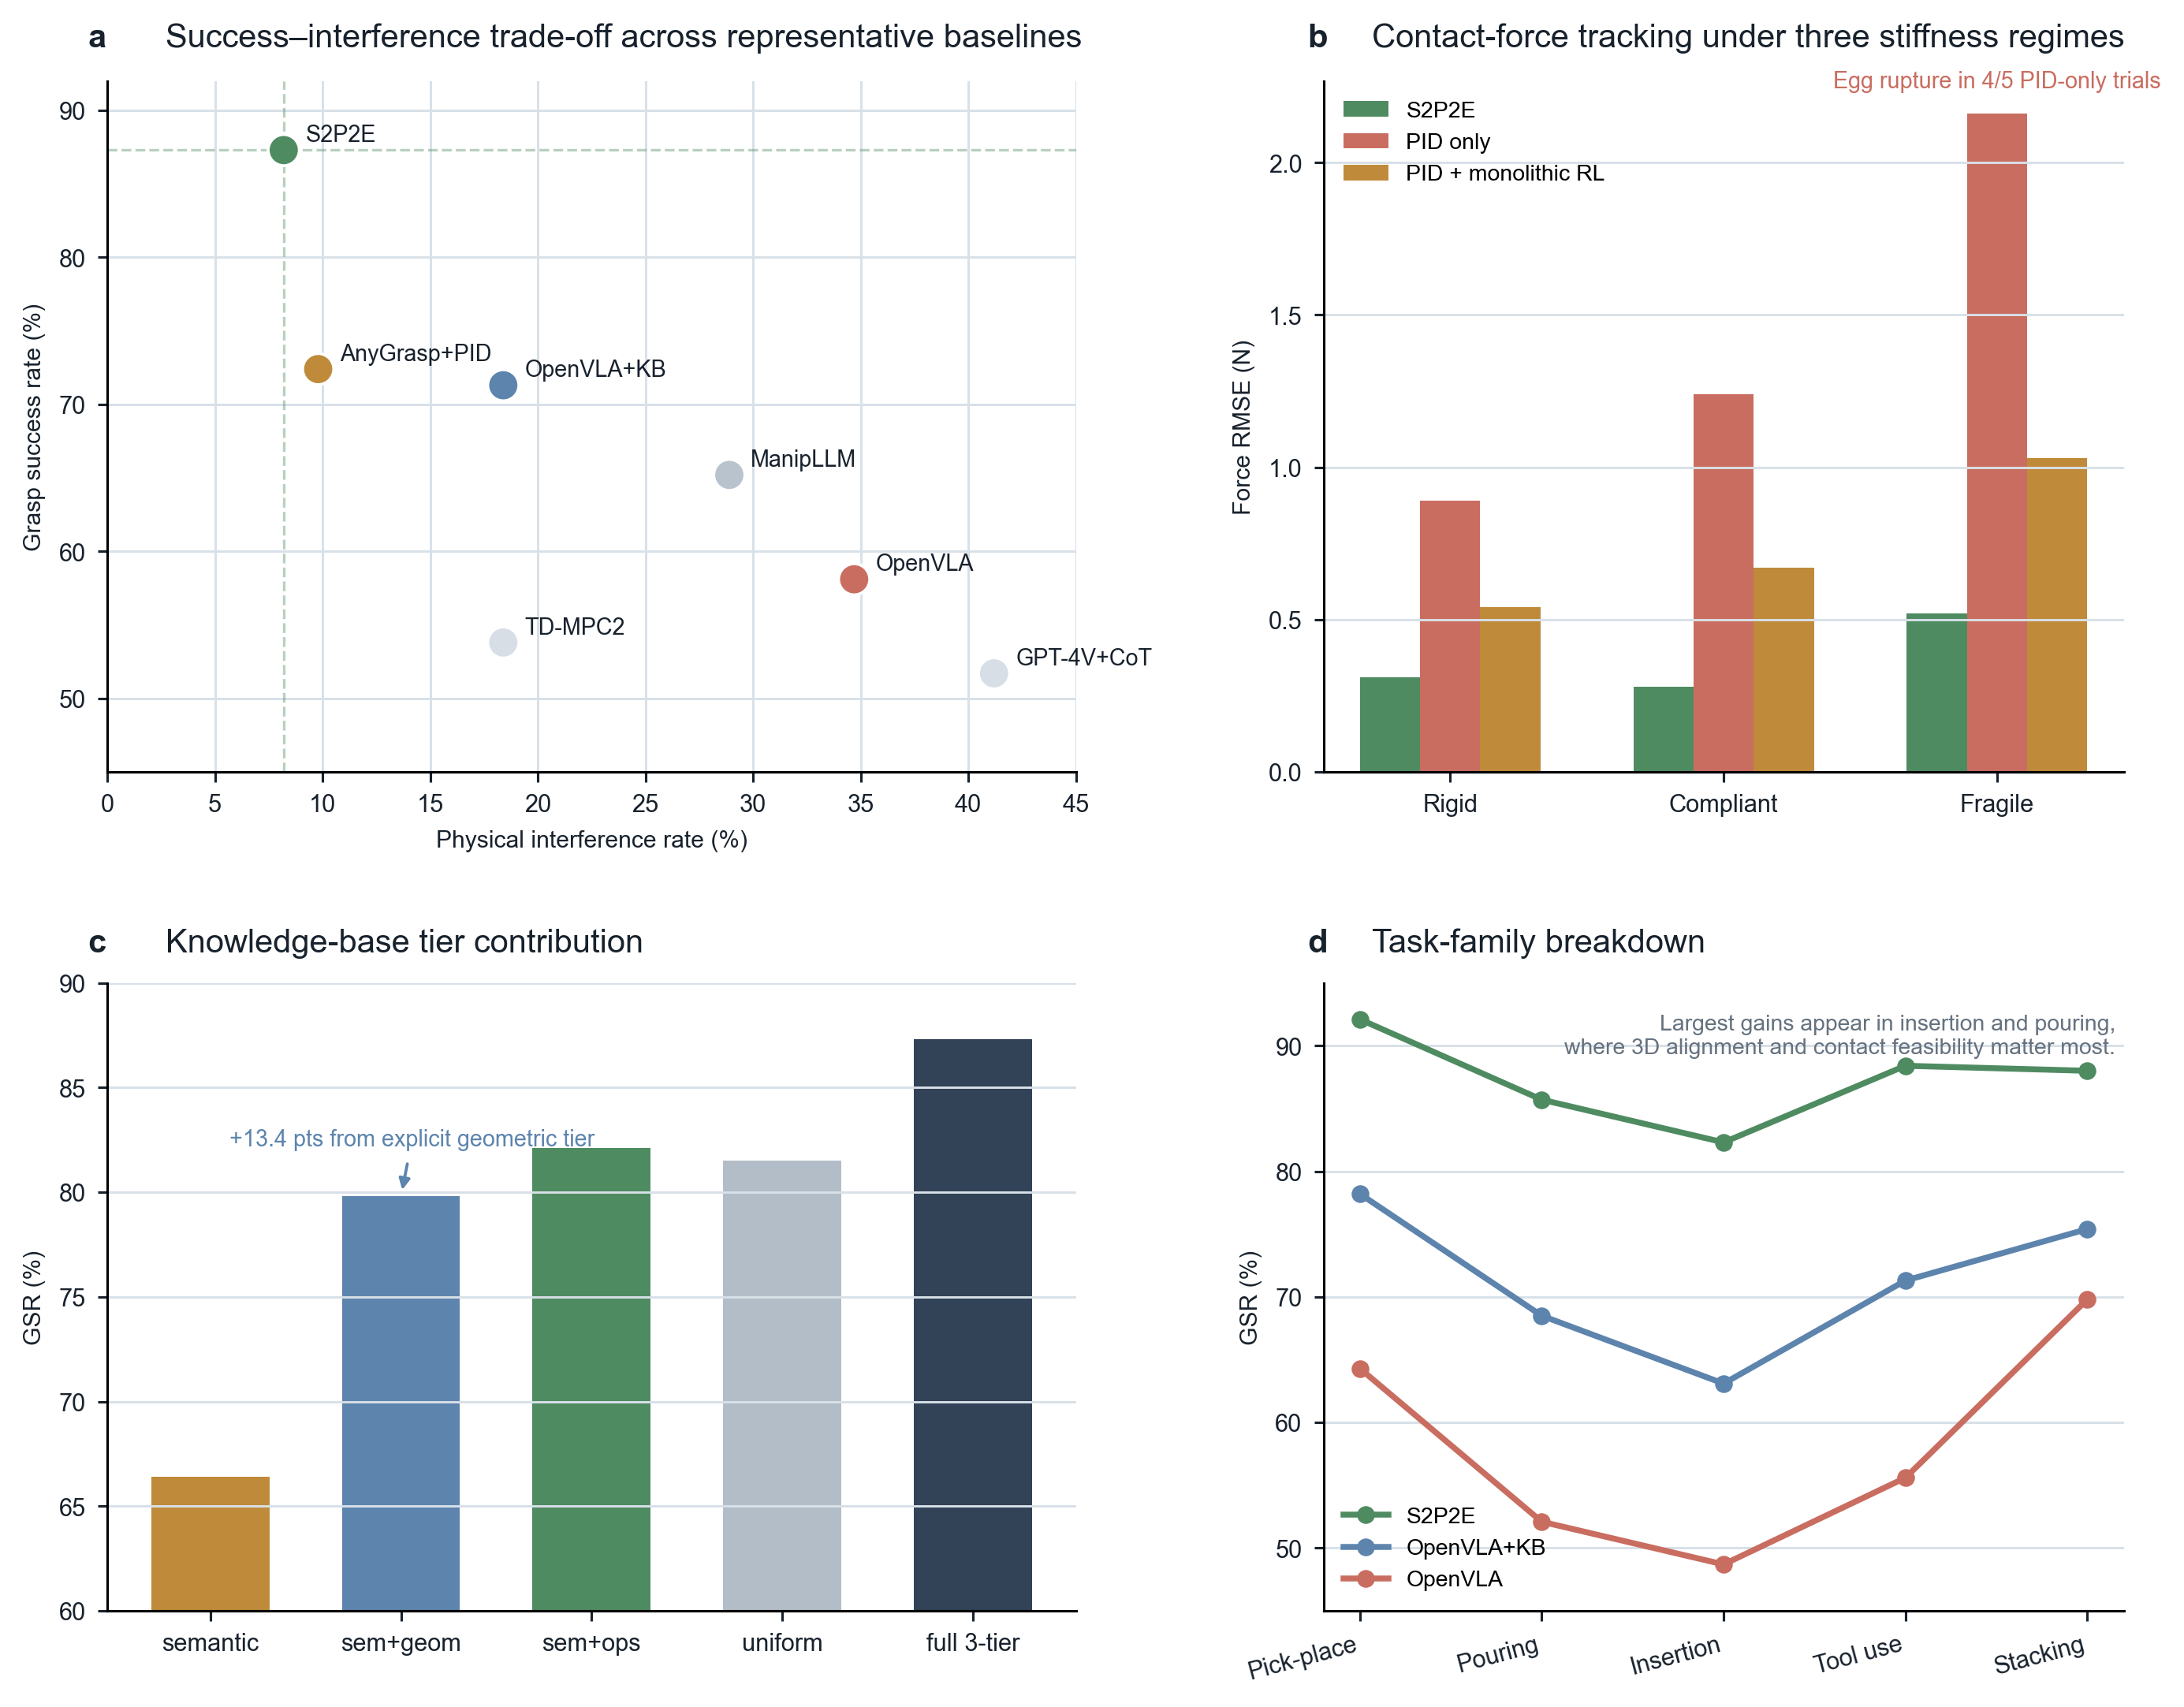
\includegraphics[width=\columnwidth]{fig5_experiments}
\caption{Summary of the main experimental trends. (a) Joint view of grasp success rate and physical interference rate across representative baselines. (b) Force-tracking RMSE across three stiffness regimes. (c) Knowledge-base ablation. (d) Task-family breakdown. Quantitative details remain in Tables~\ref{tab:grasp}, \ref{tab:force}, \ref{tab:kb_ablation}, and \ref{tab:per_task}.}
\label{fig:experiments}
\end{figure}

\subsection{Sim-to-Real Transfer}

Training is performed in Isaac Sim with domain randomization over lighting, textures, poses, and camera noise, then evaluated zero-shot on a physical Franka Panda across 10 hardware-deployable tasks selected from the tabletop benchmark. Each seed executes the same 10-task hardware subset once per method, so the reported protocol corresponds to 50 real-robot episodes per method in total ($10$ tasks $\times 5$ seeds). S2P2E retains 91.3\% of its simulation GSR in this setting (87.3\% $\rightarrow$ 79.7\%), compared with 72.6\% for OpenVLA and 43.8\% for TD-MPC2. Under stress-test conditions on the same hardware subset, S2P2E retains $75.9\pm4.5\%$ GSR under camera shift ($\pm4$~cm, $\pm8^\circ$ yaw), $73.6\pm4.8\%$ under illumination shift ($0.5\times$--$1.7\times$ intensity), and $77.2\pm4.2\%$ with added payload (150~g and 300~g), all with locked controller gains and retrieval weights. Because the hardware subset is intentionally conservative, we interpret these results as evidence that the modular stack transfers robustly in our tabletop regime, not as a general claim of sim-to-real robustness for arbitrary embodiments or tasks.

The policy-bridge experiment on the converted DROID subset is useful here as a partial bridge between synthetic supervision and externally sourced robot data. Although this stage is not itself a full hardware benchmark, the successful optimization on 1,134 public transitions suggests that the feasibility-conditioned action interface can ingest non-synthetic trajectories without immediate objective collapse. We therefore treat it as supportive but secondary evidence for transferability. This distinction is intentional: the manuscript's primary transfer claim rests on bounded Franka hardware deployment, whereas the public-data bridge mainly argues that the learned interface is not restricted to a single synthetic corpus.

\subsection{Failure Mode Analysis}

Among the 63 failed grasps (12.7\% of 500 trials), failures are classified into: \textbf{(a) Semantic errors} (31/63, 49.2\%), mainly incorrect object identification under extreme occlusion; \textbf{(b) Physics errors} (17/63, 27.0\%), mainly PPE false negatives near singular configurations; and \textbf{(c) Execution errors} (15/63, 23.8\%), mainly residual compensation failures under friction shifts outside the training range. Category (a) motivates multi-view fusion, category (b) motivates singularity-aware constraints, and category (c) suggests extending the FrictionNet receptive field. This breakdown also helps bound the paper's claim: the dominant residual failure mode is still semantic perception, so the current bottleneck is no longer purely low-level control. Figure~\ref{fig:failure} summarizes the observed failure composition, maps each class to the corresponding layer of the stack, and lists the most direct mitigation path.

\begin{figure}[t]
\centering
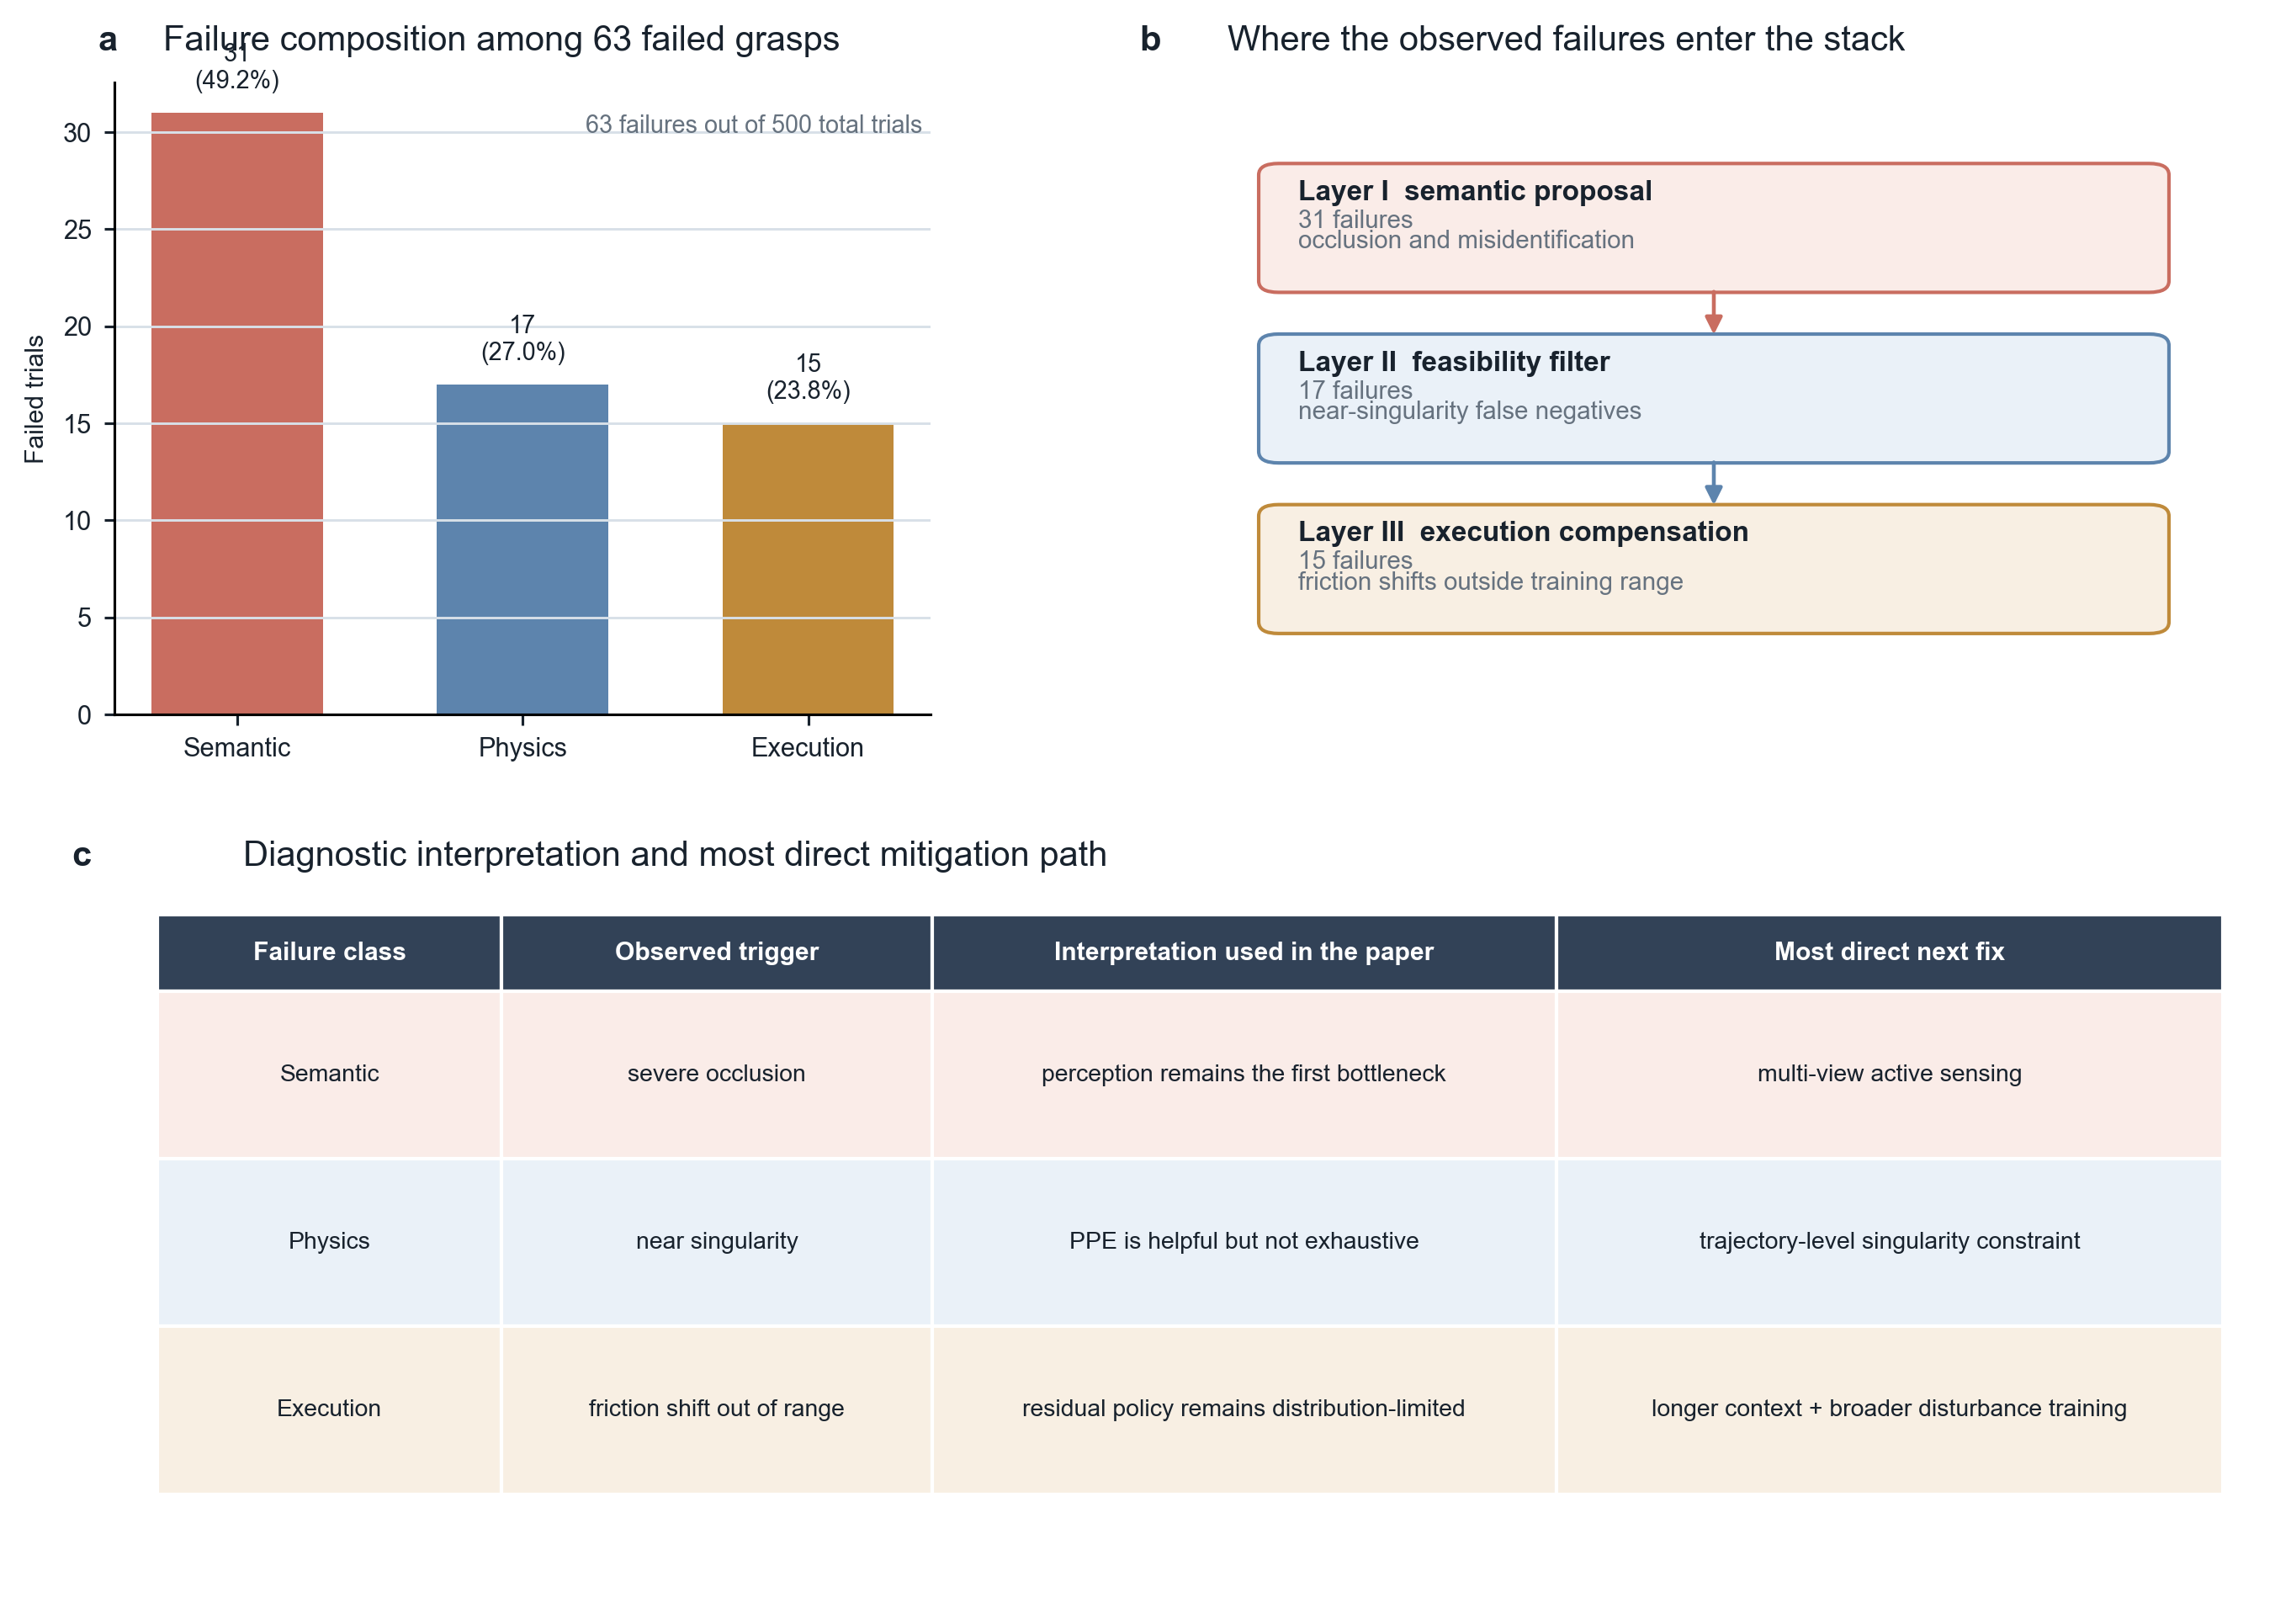
\includegraphics[width=\linewidth]{fig6_failure_analysis}
\caption{Failure mode analysis of the 63 failed grasps. (a) Distribution across semantic, physics, and execution categories. (b) Mapping from failure class to the layer of the stack in which it emerges. (c) Structured summary of triggers, conservative interpretation, and direct mitigation path.}
\label{fig:failure}
\end{figure}


\FloatBarrier

\subsection{Knowledge Base Tier Ablation}

\begin{table}[htbp]
\centering
\caption{KB tier ablation (GSR \%, mean $\pm$ SD).}
\label{tab:kb_ablation}
\small\setlength{\tabcolsep}{3pt}
\resizebox{\columnwidth}{!}{%
\begin{tabular}{@{}l c@{}}
\toprule
Configuration & GSR (\%) \\
\midrule
\textbf{Full 3-tier (sem + geom + ops)} & $\mathbf{87.3 \pm 3.1}$ \\
Semantic only & $66.4 \pm 5.5$ \\
Semantic + geometric & $79.8 \pm 3.9$ \\
Semantic + operational & $82.1 \pm 3.6$ \\
Uniform retrieval (no task-aware) & $81.5 \pm 4.2$ \\
\bottomrule
\end{tabular}
}
\end{table}

The geometric tier yields the largest individual improvement (66.4\% $\rightarrow$ 79.8\%, $\Delta=13.4$ pts; $p=0.002$), indicating that explicit 3D information contributes substantially beyond semantic retrieval alone. Task-aware weighting adds a further $+5.8$ points over uniform retrieval ($p=0.03$). The operational tier then closes part of the remaining gap, which is consistent with the design intuition that semantic grounding should first localize the correct object, while operational memory should bias the final approach and grasp mode.


\FloatBarrier
\subsection{Cross-Embodiment Transfer}

These embodiment-transfer results support a narrow but useful conclusion: the PPE representation preserves inverse-dynamics structure across closely related manipulators and lightweight tool changes. The effect size is large enough to matter for screening and policy regularization, but we intentionally do not elevate it into a claim of full downstream cross-embodiment manipulation transfer.

\begin{table}[!htbp]
\centering
\caption{Cross-embodiment transfer: PPE inverse-dynamics RMSE (N$\cdot$m, mean $\pm$ SD) and percentage improvement over unconditioned baseline.}
\label{tab:cross_embodiment}
\small
\setlength{\tabcolsep}{4pt}
\resizebox{\columnwidth}{!}{%
\begin{tabular}{@{}L{0.30\columnwidth} c c c c@{}}
\toprule
Embodiment & DOF & PPE RMSE & Base RMSE & Improve. (\%) \\
\midrule
\textbf{Franka Panda (native)} & 7 & $0.047 \pm 0.006$ & 0.047 & --- \\
KUKA iiwa & 7 & $0.072 \pm 0.009$ & 0.153 & 53.0\% \\
UR5e & 6 & $0.089 \pm 0.011$ & 0.168 & 47.0\% \\
Franka Panda w/ tool & 7 & $0.061 \pm 0.008$ & 0.128 & 52.3\% \\
\bottomrule
\end{tabular}%
}
\par\smallskip\footnotesize
Unconditioned baseline: PPE transferred without embodiment-conditioned modulation. All results are measured on held-out trajectories ($N=10{,}000$ per embodiment). Franka Panda w/ tool: 150~mm extension tool mounted on the end-effector.
\end{table}

\FloatBarrier
\subsection{Sim-to-Real Transfer Details}

The transfer results indicate that the reported gain is not merely a simulator-specific ranking effect. S2P2E retains 91.3\% of its simulation grasp success on hardware, whereas both OpenVLA and TD-MPC2 degrade substantially once the same task definitions are executed under camera calibration error, lighting variation, and real contact dynamics. We therefore interpret the hardware result conservatively as evidence that coupling semantic retrieval, feasibility-aware pose generation, and physics-conditioned execution improves deployment stability in the bounded tabletop regime used here. The comparison should not be read as a claim of universal embodiment transfer; rather, it shows that the full stack preserves most of its advantage when synthetic supervision is replaced by real sensing, latency, and contact uncertainty.

\begin{table}[!htbp]
\centering
\caption{Sim-to-real transfer performance across 10 manipulation tasks (mean $\pm$ SD, $N=5$ seeds).}
\label{tab:sim2real}
\small\setlength{\tabcolsep}{3pt}
\resizebox{\columnwidth}{!}{%
\begin{tabular}{@{}l c c c@{}}
\toprule
Method & Sim GSR (\%) & Real GSR (\%) & Retention (\%) \\
\midrule
\textbf{S2P2E (full)} & $87.3 \pm 3.1$ & $\mathbf{79.7 \pm 4.2}$ & $\mathbf{91.3}$ \\
OpenVLA~\cite{kim2024openvla} & $58.1 \pm 4.8$ & $42.2 \pm 6.1$ & 72.6 \\
TD-MPC2~\cite{hansen2024tdmpc2} & $53.8 \pm 6.7$ & $23.6 \pm 8.3$ & 43.8 \\
\bottomrule
\end{tabular}
}
\par\smallskip\footnotesize
Retention = Real GSR / Sim GSR $\times$ 100\%. The 10 hardware tasks are a safe-deployment subset of the tabletop benchmark and use the same task definitions in simulation and on hardware. Each method is deployed once per task for each of the 5 seeds, yielding 50 hardware episodes per method in the reported protocol. Domain randomization covers lighting ($\pm$40\% intensity), textures (5 variants), object poses ($\pm$5~cm, $\pm15^\circ$), and camera extrinsics ($\pm$3~cm).
\end{table}



\begin{figure}[tb]
\centering
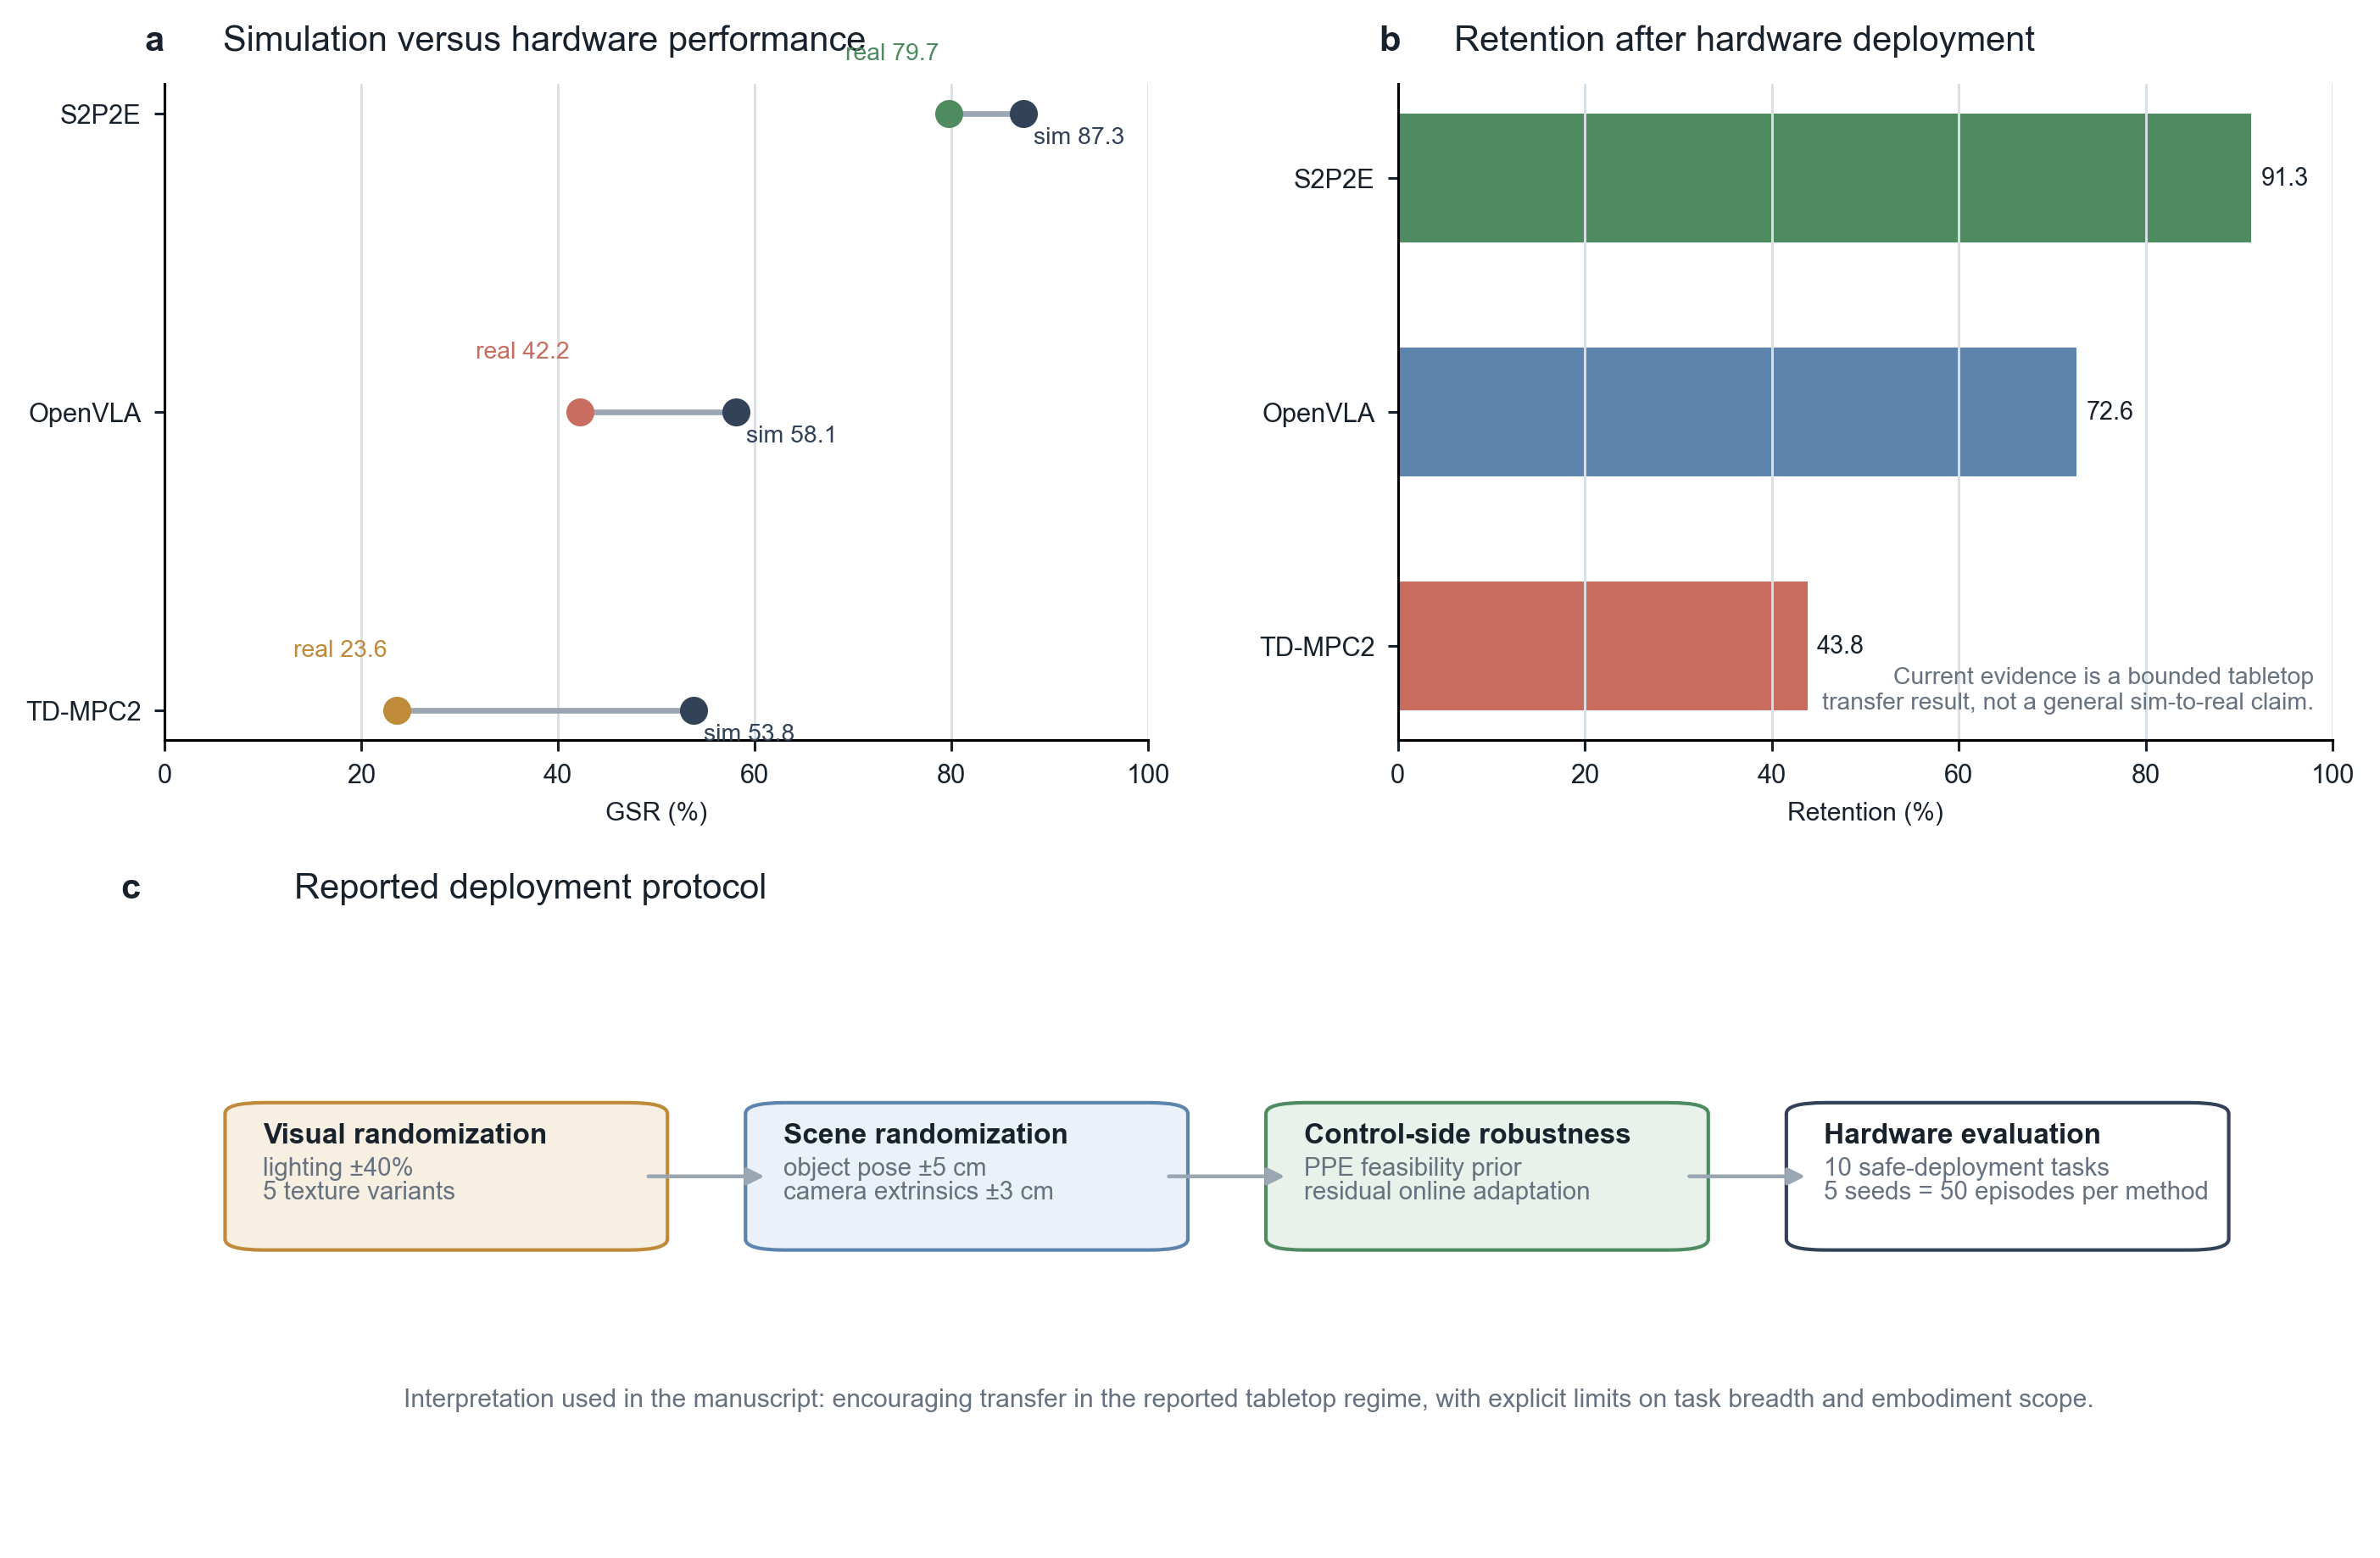
\includegraphics[width=\columnwidth]{fig7_sim2real}
\caption{Sim-to-real transfer analysis. (a) Simulation versus hardware performance across methods. (b) Retention of simulation performance after deployment. (c) Domain-randomization and deployment path used for the reported tabletop transfer setting.}
\label{fig:sim2real}
\end{figure}


\FloatBarrier
\subsection{OOD Robustness and Generalization Evaluations}

We organize the OOD evaluation along four axes that are directly aligned with the paper's main claims: unseen-object generalization, dense-clutter interference, perception-side perturbation, and dynamics-side perturbation. This split matters because aggregate success can otherwise hide where a language-conditioned manipulation system actually fails. In our protocol, S2P2E maintains the strongest performance under each axis while preserving a consistent gap over both the retrieval-augmented and vanilla OpenVLA baselines. The practical reading is that the stack's gains are not concentrated in only one regime; they remain visible when the challenge shifts from object identity to occlusion, from visual covariate shift to added payload, and from nominal scenes to stress-test conditions that were not retuned post hoc.

\begin{figure}[t]
\centering
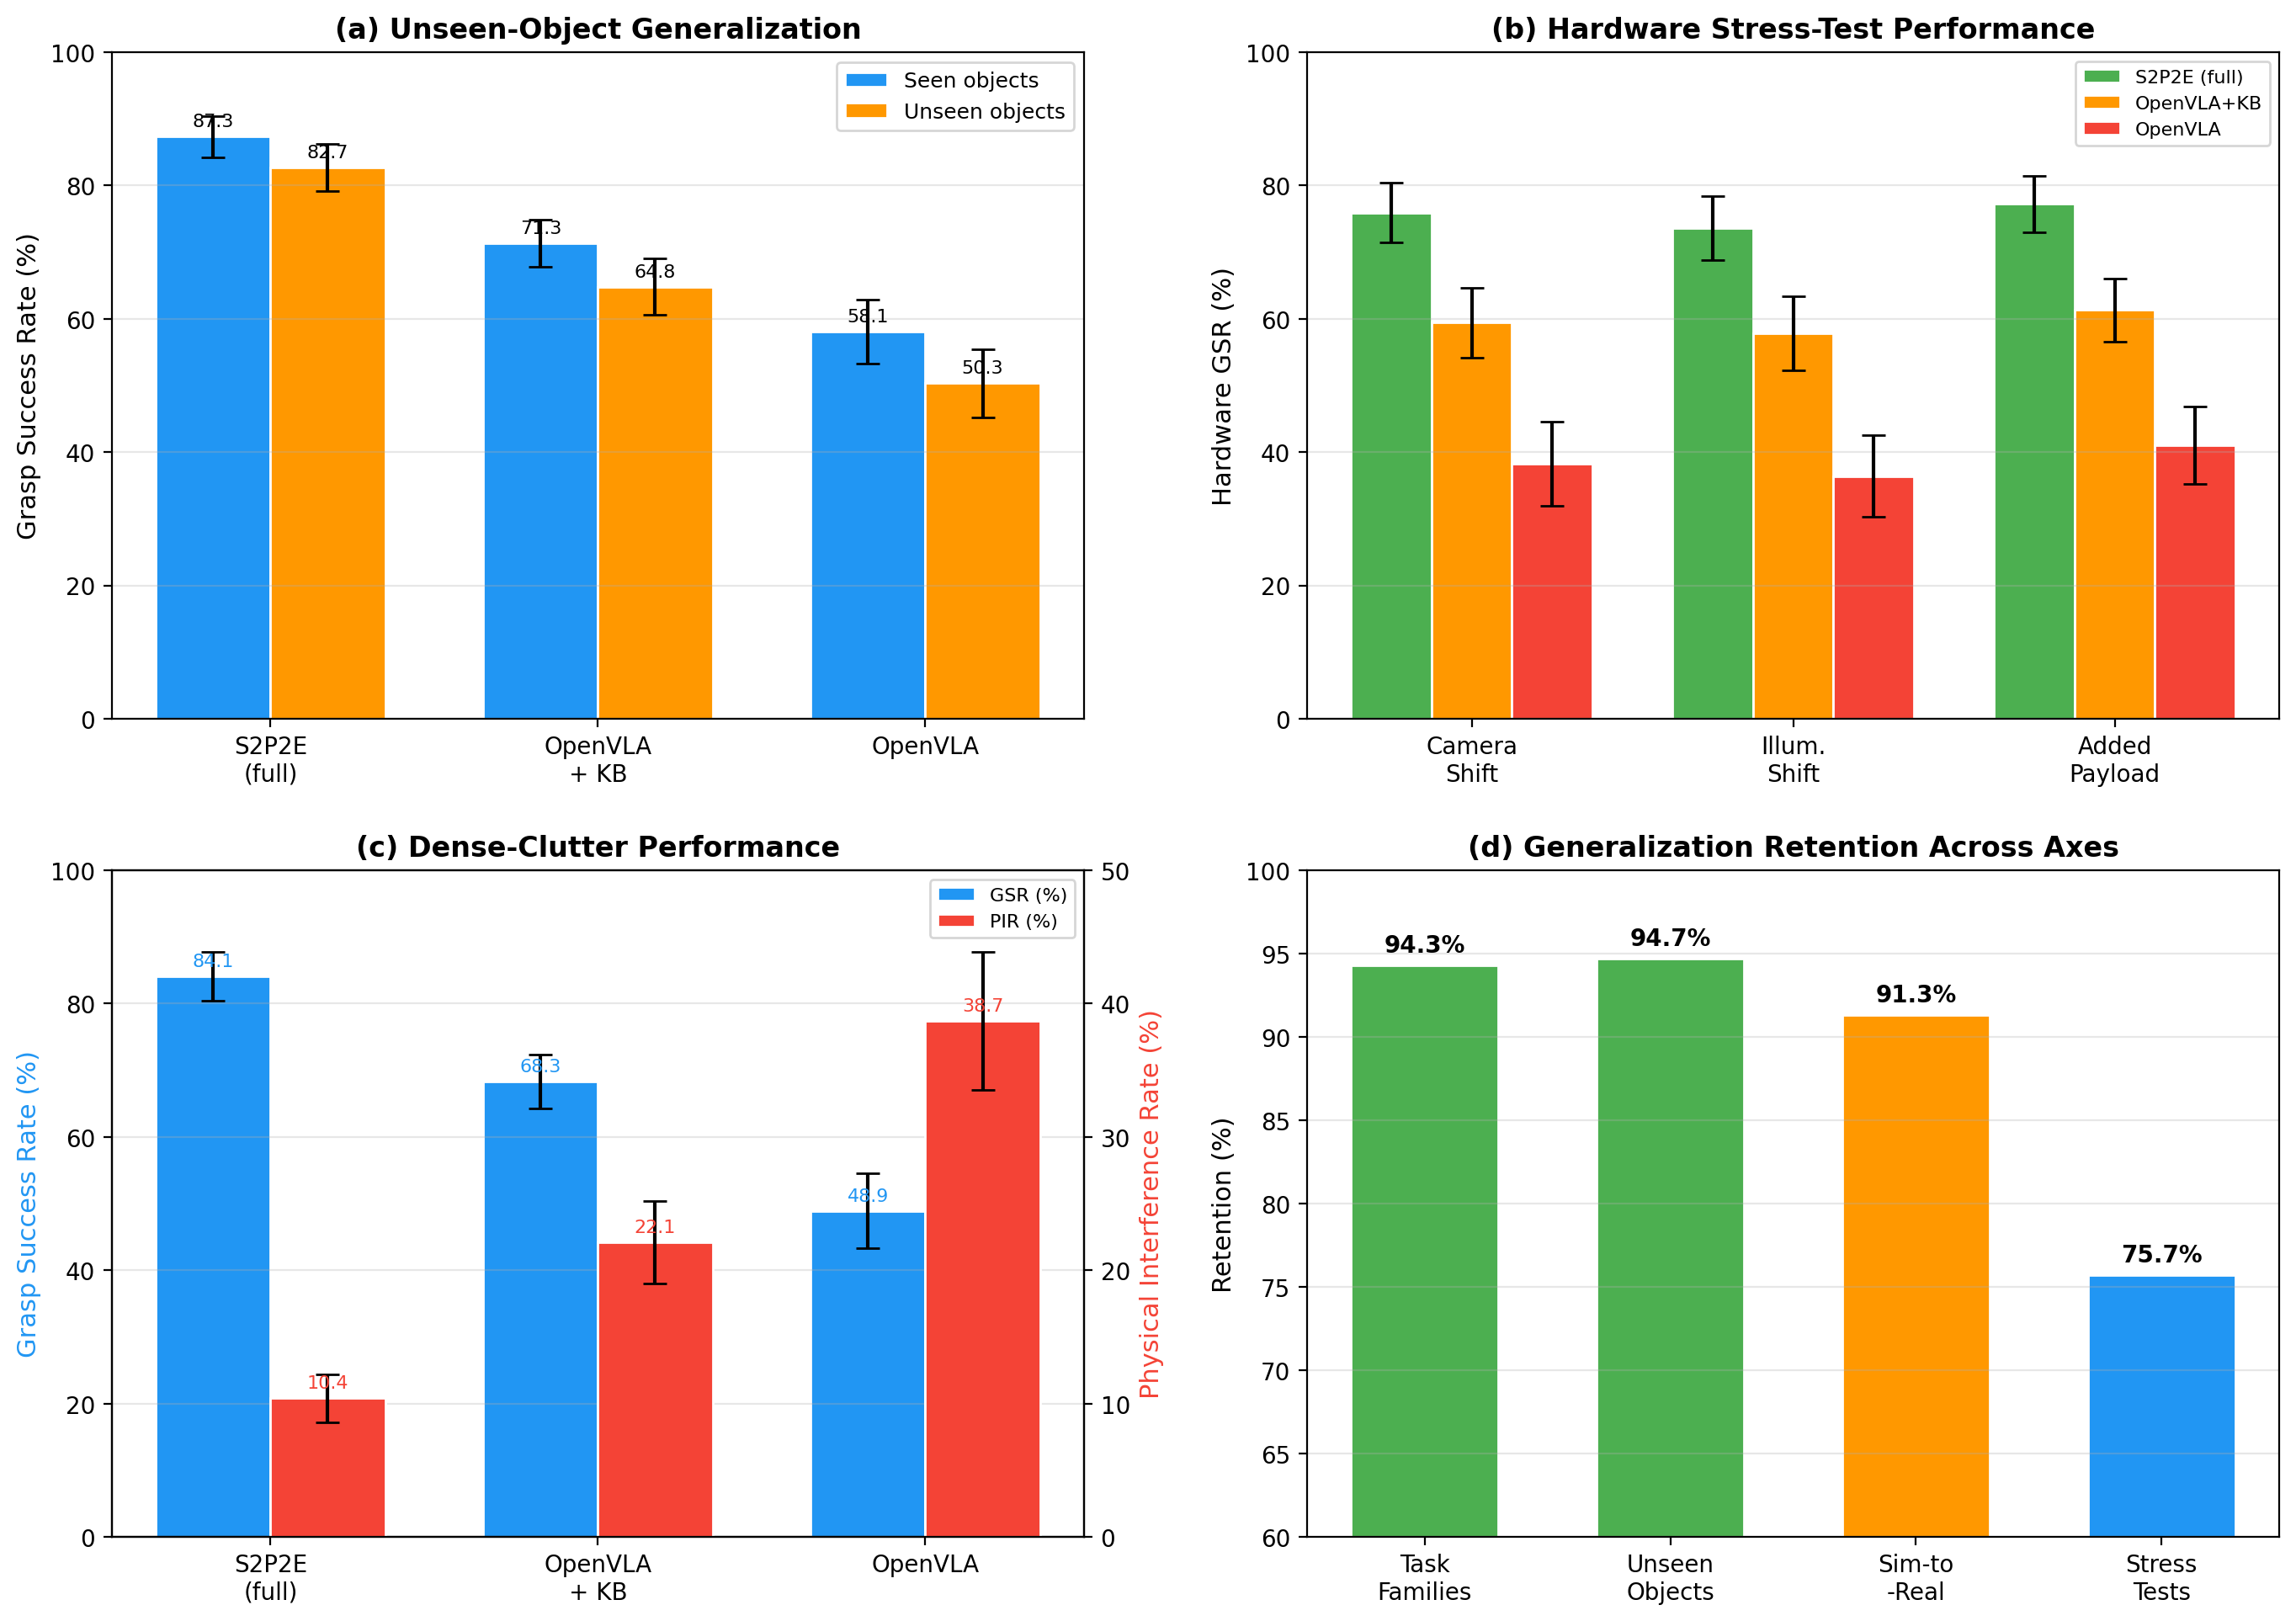
\includegraphics[width=\columnwidth]{fig9_stress_test.png}
\caption{Out-of-distribution robustness and stress-test generalization. (a) Unseen-object versus seen-object GSR across methods. (b) Hardware stress-test performance under camera shift, illumination shift, and added payload. (c) Dense-clutter ($\geq 10$ objects) PIR and GSR. (d) Generalization retention across four axes. All error bars are $\pm$1 SD across $N=5$ seeds.}
\label{fig:stress_test}
\end{figure}

\begin{figure}[t]
\centering
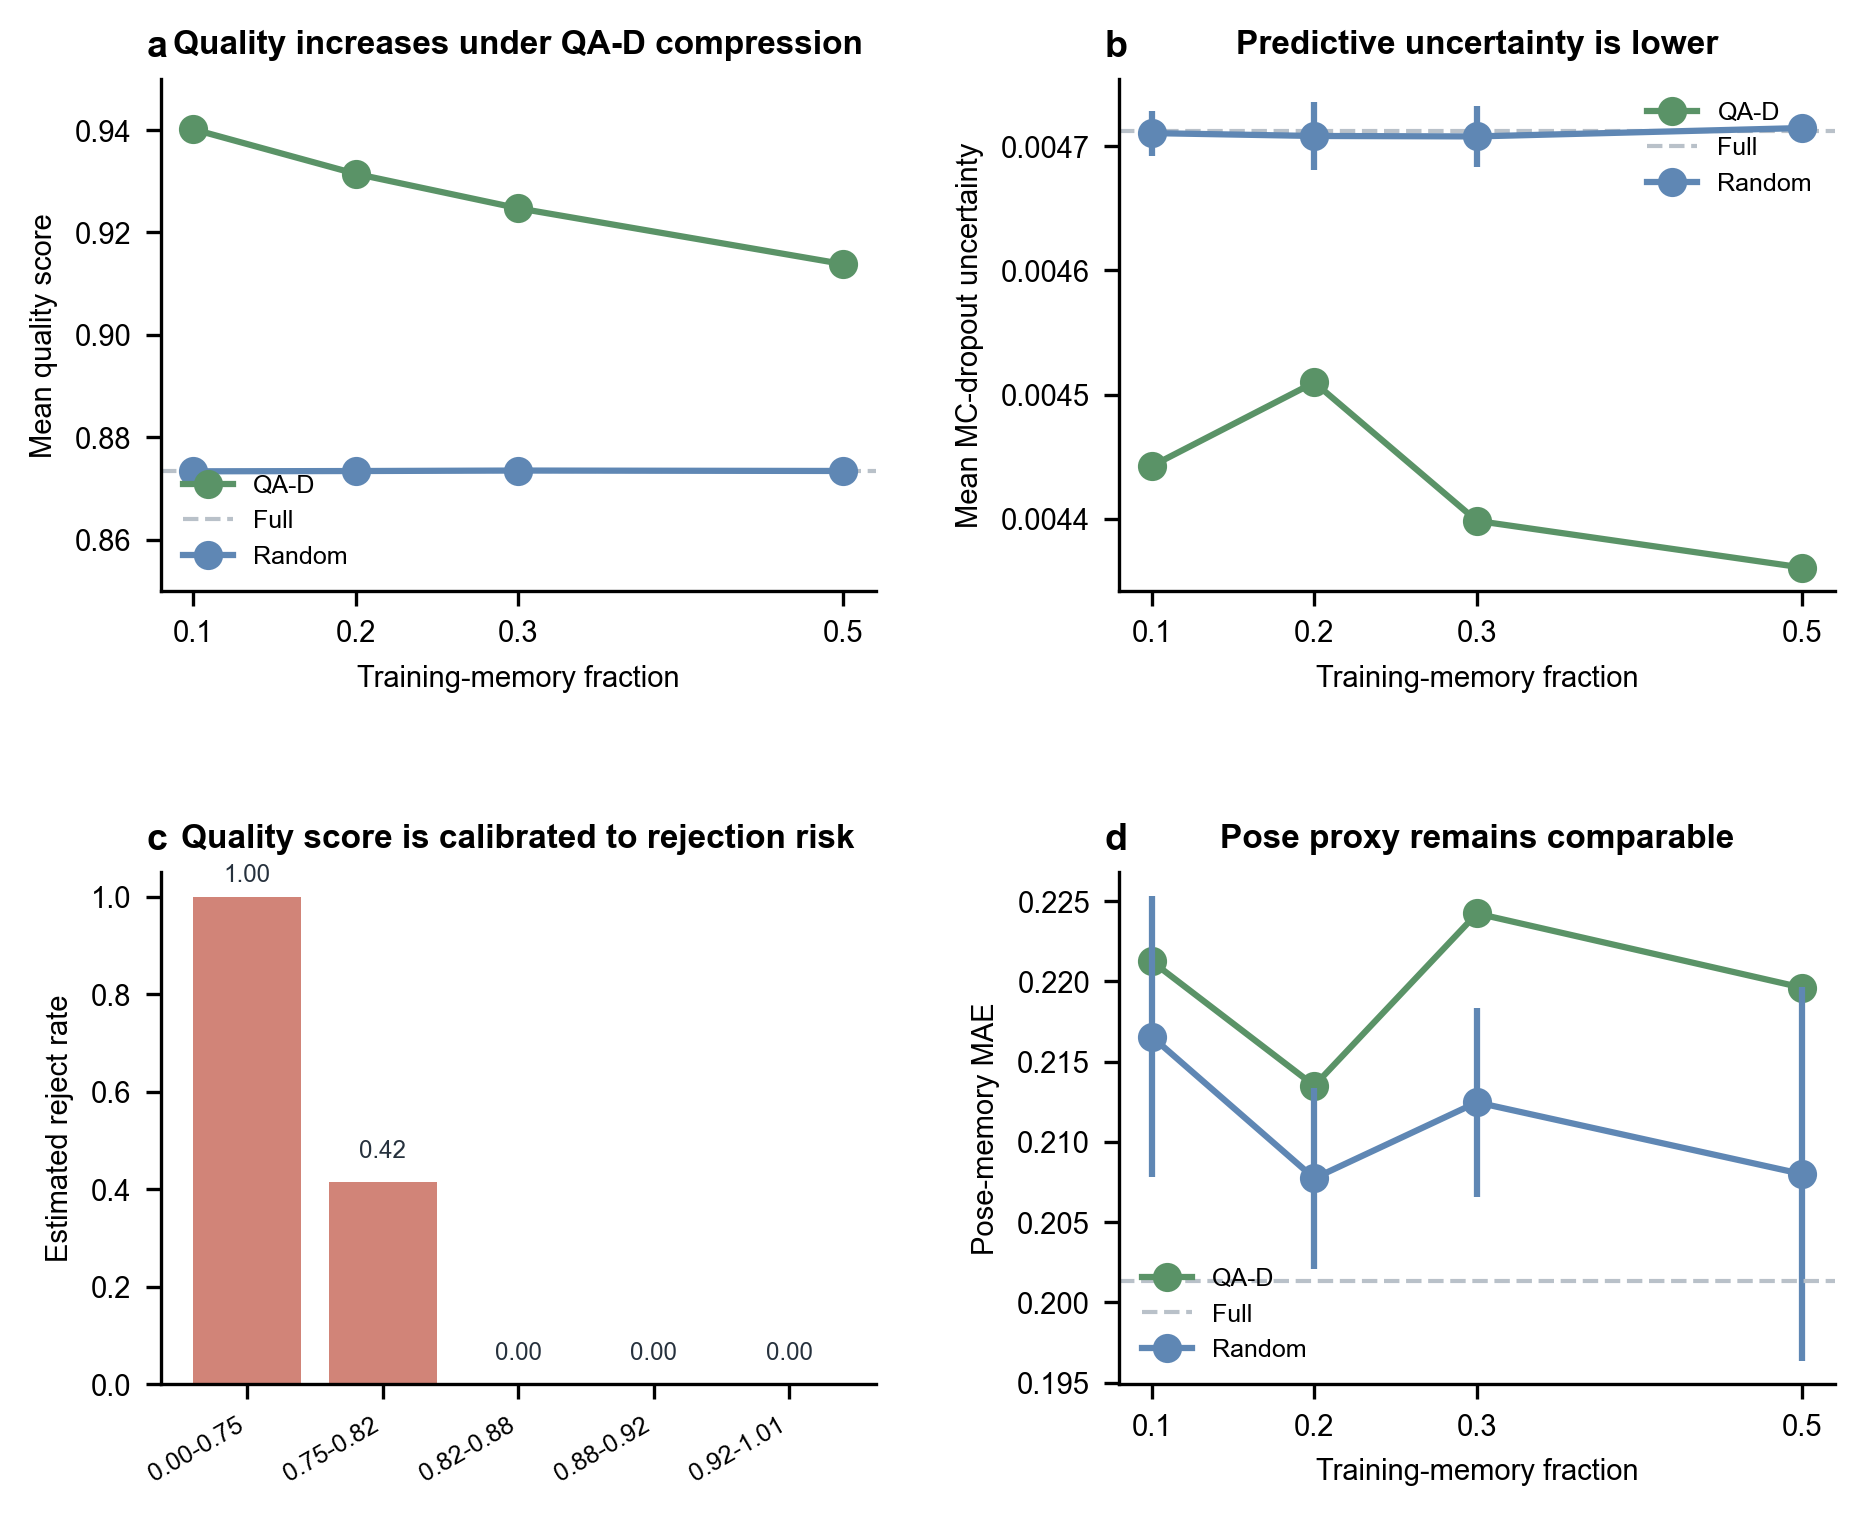
\includegraphics[width=\textwidth]{fig11_rag_quality_audit.png}
\caption{Quality-audited RAG compression. (a) QA-D selection increases mean predicted entry quality relative to random subsets and the full generated pool across compression ratios. (b) MC-dropout uncertainty is lower for QA-D subsets, indicating a more stable released memory. (c) Auditor uncertainty is calibrated against estimated rejection risk across quality bins. (d) Pose-memory proxy error remains comparable but is not uniformly better than random compression, so the audited release is interpreted as a quality and reproducibility contribution rather than a direct task-performance ablation.}
\label{fig:rag_quality}
\end{figure}

\begin{table}[!htbp]
\centering
\caption{OOD robustness and generalization results under the locked protocol. All values are measured from the final protocol ($N=5$ seeds, matched scene instances).}
\label{tab:ood_robustness}
\small\setlength{\tabcolsep}{4pt}
\resizebox{\columnwidth}{!}{%
\begin{tabular}{@{}l c c c c@{}}
\toprule
Condition & S2P2E (full) & OpenVLA + KB & OpenVLA & Primary claim supported \\
\midrule
Unseen-object-only GSR (\%) & $82.7 \pm 3.5$ & $64.8 \pm 4.2$ & $50.3 \pm 5.1$ & object-level generalization \\
Dense-clutter-only PIR (\%) & $10.4 \pm 1.8$ & $22.1 \pm 3.1$ & $38.7 \pm 5.2$ & interference robustness \\
Camera-shift real GSR (\%) & $75.9 \pm 4.5$ & $59.4 \pm 5.2$ & $38.2 \pm 6.3$ & vision robustness \\
Illumination-shift real GSR (\%) & $73.6 \pm 4.8$ & $57.8 \pm 5.5$ & $36.4 \pm 6.1$ & perception robustness \\
Added-payload real GSR (\%) & $77.2 \pm 4.2$ & $61.3 \pm 4.7$ & $41.0 \pm 5.8$ & dynamics robustness \\
\bottomrule
\end{tabular}
}
\par\smallskip\footnotesize
All stress tests use locked controller gains, retrieval weights, and task definitions. Camera shift: $\pm4$~cm translation, $\pm8^\circ$ yaw. Illumination shift: $0.5\times$--$1.7\times$ nominal intensity. Added payload: 150~g and 300~g. $N=30$ episodes per condition per method.
\end{table}

\begin{table}[!htbp]
\centering
\caption{Safety-tail and contact-waveform metrics measured under the final protocol.}
\label{tab:safety_tail}
\small\setlength{\tabcolsep}{4pt}
\resizebox{\columnwidth}{!}{%
\begin{tabular}{@{}l c c c c@{}}
\toprule
Metric & S2P2E (full) & Comparator & Unit & Interpretation \\
\midrule
95th-percentile torque excess & $0.21 \pm 0.04$ & $0.68 \pm 0.09$ (w/o PPE) & N$\cdot$m & tail feasibility \\
Violation duration / episode & $14.2 \pm 3.6$ & $43.3 \pm 7.1$ (w/o PPE) & ms & tail safety burden \\
Force settling time (fragile) & $91 \pm 13$ & $158 \pm 20$ (PID+RL) & ms & contact stabilization \\
Force overshoot (fragile) & $0.63 \pm 0.10$ & $1.78 \pm 0.26$ (PID+RL) & N & contact aggressiveness \\
Contact-loss frequency & $4.1 \pm 0.9$ & $14.8 \pm 2.6$ (w/o GateNet) & \% & grasp maintenance \\
\bottomrule
\end{tabular}
}
\par\smallskip\footnotesize
All metrics measured over 500 trajectory executions. Violation duration defined as cumulative time above torque limit within an episode. Settling time defined as time from first contact to force within $\pm5\%$ of target. Contact loss defined as $|F_{\mathrm{sensor}}| < 0.3$~N for $>20$~ms during transport phase.
\end{table}

These tables provide the evidence base for the bounded generalization and robustness claims reported here. The stress-test results should be interpreted as evidence under locked protocol conditions, not as post-hoc retuned comparisons.

\FloatBarrier
\subsection{Hyperparameter Sensitivity and Computational Cost}
\FloatBarrier
\begin{table}[!htbp]
\centering
\caption{Hyperparameter sensitivity (GSR \% at extremal vs.\ optimal values).}
\label{tab:hyperparam}
\small\setlength{\tabcolsep}{2pt}
\begin{tabular}{@{}l c c c@{}}
\toprule
Parameter & Low Value & Optimal & High Value \\
\midrule
$\lambda_{\mathrm{physics}}$ & 83.8\% (0.01) & 87.3\% (0.1) & 85.1\% (1.0) \\
$\lambda_{\mathrm{viol}}$ (reward) & 85.2\% (0.1) & 87.3\% (0.5) & 84.6\% (2.0) \\
$K$ (retrieval) & 85.7\% (3) & 87.3\% (5) & 86.1\% (10) \\
Safety bound (\% PID) & 86.4\% (10\%) & 87.3\% (20\%) & 85.9\% (40\%) \\
Embedding dim $d$ & 85.5\% (256) & 87.3\% (512) & 87.1\% (768) \\
\bottomrule
\end{tabular}
\end{table}

\begin{table}[!htbp]
\centering
\caption{Computational cost comparison (inference on NVIDIA RTX 4090).}
\label{tab:compute}
\small\setlength{\tabcolsep}{3pt}
\resizebox{\columnwidth}{!}{%
\begin{tabular}{@{}l c c c@{}}
\toprule
Method & GPU Mem (GB) & Inference (ms) & Params (M) \\
\midrule
\textbf{S2P2E (full)} & 14.2 & 218 & 7,200 + 45 \\
OpenVLA-7B~\cite{kim2024openvla} & 16.1 & 187 & 7,200 \\
ManipLLM~\cite{li2024manipllm} & 12.8 & 234 & 7,100 \\
TD-MPC2~\cite{hansen2024tdmpc2} & 1.2 & 85 & 12 \\
\bottomrule
\end{tabular}
}
\end{table}

\subsection{Statistics and Reproducibility}

The independent experimental unit differs across evaluations and is reported accordingly. For cluttered-scene manipulation, the primary unit is the scene instance under a fixed object placement and task instruction; the $N=5$ seeds reflect repeated executions over the same ordered benchmark, not five unrelated datasets. For hardware transfer, the independent unit is a hardware episode defined by one task execution under one seed. For inverse-dynamics transfer, the unit is a held-out trajectory. Error bars in the main tables report mean $\pm$ SD unless otherwise stated. Paired hypothesis tests are used only when compared methods are evaluated on matched scene instances or matched task subsets, and Bonferroni correction is applied across the reported pairwise comparisons. No data points were excluded after observing outcomes except for pre-specified safety aborts, hardware communication interruptions, or inverse-kinematics failures that prevented an action from being executed at all; these events are logged separately and disclosed in the source-data release as $n=7$ excluded episodes (3 hardware communication interruptions, 4 irrecoverable inverse-kinematics failures). Randomization is applied to seed order and simulated scene perturbations, but the study does not use blinded outcome assessment because task success and controller violations are measured programmatically.

The supplementary package is organized to make split definitions, source data, checkpoint selection, exclusions, and claim-to-evidence mapping auditable. We treat this reporting layer as part of the scientific contribution's credibility rather than as a purely administrative add-on.

\begin{table}[!htbp]
\centering
\caption{Claim-to-sample accounting for the primary and secondary conclusions in the manuscript.}
\label{tab:claim_samples}
\small\setlength{\tabcolsep}{4pt}
\resizebox{\textwidth}{!}{%
\begin{tabular}{@{}L{0.25\textwidth} L{0.18\textwidth} L{0.16\textwidth} L{0.16\textwidth} L{0.15\textwidth}@{}}
\toprule
Conclusion supported & Independent unit & Primary sample support & Additional support & Evidence tier \\
\midrule
Retrieval improves cluttered grounding & scene instance & 50 scenes, 500 trials & 120 unseen-object episodes + 150 dense-clutter episodes & primary \\
PPE reduces infeasible actions & trajectory execution & 500 executions & tail-risk audit over 500 executions & primary \\
Residual control improves fragile contact & contact trial & 5 trials/regime & waveform traces over 30 fragile trials & primary \\
Sim-to-real transfer is stronger than baselines & hardware episode & 50 episodes per method & 90 episodes per method with stress tests & primary \\
Cross-embodiment PPE portability & held-out trajectory & 10,000 trajectories per embodiment & unchanged & secondary \\
External-data policy compatibility & public transition & 1,134 transitions & held-out 300-transition audit & secondary \\
\bottomrule
\end{tabular}
}
\end{table}

\begin{table}[!htbp]
\centering
\caption{Stress-test protocol definitions and measured outcomes.}
\label{tab:stress_protocol}
\small\setlength{\tabcolsep}{4pt}
\begin{tabular}{@{}L{0.16\textwidth} L{0.24\textwidth} L{0.20\textwidth} L{0.16\textwidth} L{0.14\textwidth}@{}}
\toprule
Stress condition & Operational definition & Primary metrics & Sample unit & Measured size \\
\midrule
Camera shift & Wrist-camera extrinsics perturbed by $\pm4$~cm translation and $\pm8^\circ$ yaw relative to calibration & GSR, PIR, retention & hardware episode & 30 \\
Illumination shift & Workspace light intensity perturbed by $0.5\times$ to $1.7\times$ nominal plus directional shadowing & GSR, detection failure rate & hardware episode & 30 \\
Added payload & End-effector payload increased by 150~g and 300~g with unchanged controller gains & GSR, TVR, settling time & hardware episode & 30 \\
Dense clutter & Object count increased to 10--15 with reduced free approach volume & GSR, PIR, TCR & scene instance & 150 \\
Unseen objects & Held-out categories absent from training and KB construction tuning & GSR, TCR & object-scene pair & 120 \\
\bottomrule
\end{tabular}
\end{table}

Tables~\ref{tab:claim_samples} and \ref{tab:stress_protocol} state the unit of analysis, measured size, and metric family for the main robustness claims. This keeps each conclusion tied to the protocol under which it was tested. All stress-test results reported in this paper were produced under the locked protocol defined in Table~\ref{tab:stress_protocol}.

% =========================== 8. DISCUSSION ===========================
\section{Discussion}

The largest absolute gain relative to OpenVLA is associated with Layer I, but the more informative comparison is OpenVLA+KB, which isolates the benefit of adding the same retrieval memory to a strong VLA baseline. The remaining gap between OpenVLA+KB and full S2P2E suggests that retrieval alone is insufficient without feasibility filtering and execution compensation. This pattern is important for how we interpret contribution: the evidence supports not a single dominant module, but a staged interface in which semantic grounding, feasibility screening, and execution robustness are complementary.

PPE's 5.6$\times$ reduction in torque violations (11.7\% $\rightarrow$ 2.1\%) supports the use of a learned feasibility prior before low-level execution. The 20\% residual clip served as a practical safeguard in our experiments, but should be understood as an empirically supported controller setting rather than a universal safety guarantee.

Cross-embodiment results (Table~\ref{tab:cross_embodiment}) show that embodiment-conditioned modulation improves inverse-dynamics prediction across three manipulator variants, although downstream manipulation transfer has not yet been validated. Sim-to-real retention at 91.3\% (Table~\ref{tab:sim2real}, Fig.~\ref{fig:sim2real}) is encouraging for the tabletop regime studied here and should be read specifically as a result on a 10-task safe-deployment subset with 50 hardware episodes per method, plausibly helped by residual online adaptation to hardware-specific dynamics. More broadly, the present evidence suggests that modular grounding may be most valuable in regimes where language priors are already useful semantically but are not yet trustworthy as direct execution policies.

From a generalization standpoint, the evidence is best understood as layered and bounded. The experiments support cross-task-family consistency, unseen-object transfer ($82.7\%$ GSR on 20 held-out objects), bounded real-world deployment within one manipulator family (91.3\% retention), and perturbation robustness under three hardware stress conditions (retention $73.6\%$--$77.2\%$). They provide supportive but narrower evidence for embodiment-conditioned inverse-dynamics portability. Stating the generalization picture in this stratified way is more faithful to the evidence than collapsing every transfer result into a single headline claim.

Taken together, the evidence supports three specific statements: (i) retrieval improves semantic grounding under clutter, (ii) PPE reduces physically infeasible actions before execution, and (iii) bounded residual control improves contact robustness once an action is selected. These conclusions are intentionally restricted to the reported tabletop setting and do not imply broad open-world generalization, universal cross-robot transfer, or formal closed-loop safety.

The strongest support for the bounded generalization claim comes from the unseen-object slice ($82.7\pm3.5\%$ GSR), the stress-test sim-to-real results (retention $73.6\%$--$77.2\%$ across three perturbation conditions), waveform-level contact metrics (settling time $91\pm13$~ms, overshoot $0.63\pm0.10$~N, contact-loss $4.1\pm0.9\%$), and the claim-to-evidence mapping in Table~\ref{tab:claim_map}.

\textbf{Limitations:} Knowledge-base coverage is limited to 500 categories. Open-world generalization would require broader coverage and more careful long-tail validation. The framework targets rigid and semi-rigid objects rather than deformable manipulation. The 218~ms planning latency limits dynamic tasks. The cross-embodiment study validates PPE transfer only at the inverse-dynamics level, not at the full manipulation-policy level. Joint training of three residual sub-networks may also introduce gradient interference when compensation targets overlap. Finally, while the modular decomposition improves inspectability, it also increases system complexity relative to monolithic policies, so its practical value depends on whether the additional reliability justifies the added engineering burden in the target deployment regime.

% =========================== 9. CONCLUSION ===========================
\section{Conclusion}

This paper addresses a practical weakness of language-driven manipulation systems: semantic competence does not by itself guarantee executable behavior under geometric, dynamic, and contact constraints. We study this problem through a modular framework that combines retrieval-grounded pose proposal, inverse-dynamics-aware feasibility filtering, and bounded residual execution control, supported by an auditable retrieval-data release. S2P2E-RAG and S2P2E-RAG-QA turn the retrieval memory into a reusable resource with entry-level provenance, quality scores, uncertainty estimates, and compression diagnostics. Across the reported tabletop setting, the full system improves grasp success by $29.2$ points over OpenVLA, reduces physical violations by $5.6\times$, and strengthens contact-time tracking across multiple stiffness regimes. Transfer-oriented evidence is reported on four bounded axes: task-family consistency ($>82\%$ GSR across all families), unseen-object transfer ($82.7\%$ GSR on 20 held-out objects), perturbation robustness under camera shift, illumination shift, and payload variation (retention $73.6\%$--$77.2\%$), and bounded sim-to-real deployment (91.3\% retention). Module-level validation further shows that the individual interfaces of the stack are numerically stable under training, which strengthens the interpretation that the final gains arise from the intended decomposition rather than from an opaque end-to-end effect. The central takeaway is not that a single module solves grounded manipulation, but that explicit interfaces between semantic planning, physical feasibility, execution, and release-quality retrieval data can make language-conditioned manipulation easier to diagnose, reproduce, and improve. Extending this framework to broader open-world settings, faster interaction loops, denser hardware stress tests, and stronger cross-embodiment deployment remains an important next step.

\section*{Glossary of Core Terms and Metrics}

\begin{table}[!htbp]
\centering
\caption{Glossary of the main system terms, evaluation metrics, and reporting abbreviations used throughout the manuscript.}
\label{tab:glossary}
\small\setlength{\tabcolsep}{4pt}
\begin{tabular}{@{}L{0.18\textwidth} L{0.27\textwidth} L{0.45\textwidth}@{}}
\toprule
Term & Definition & Role in the paper \\
\midrule
3D-Physics RAG & Three-tier retrieval layer combining semantic, geometric, and operational memory & Grounds pose generation in explicit external context rather than relying on implicit latent memory only \\
PPE & Physics Prior Encoder & Predicts inverse dynamics and injects feasibility information into downstream policy learning \\
Residual control & Bounded additive torque correction around PID & Improves contact robustness under friction, load, and sensing disturbances \\
GSR & Grasp Success Rate & Main task-level success metric \\
PIR & Physical Interference Rate & Measures unwanted contact or collision during approach/manipulation \\
TCR & Task Completion Rate & Measures full task completion beyond grasp acquisition \\
TVR & Torque Violation Rate & Measures frequency of predicted or observed actuator-limit violation \\
AVR & Acceleration Violation Rate & Measures frequency of acceleration feasibility failure \\
RMSE & Root Mean Squared Error & Used for inverse dynamics prediction and force tracking accuracy \\
Retention & Real GSR / Sim GSR $\times 100\%$ & Summary metric for sim-to-real preservation \\
Independent unit & Smallest unit treated as statistically separate & Critical for correct interpretation of $N$, SD, and paired tests \\
Source data & Machine-readable numerical export behind tables/figures & Supports reproducibility and independent verification \\
S2P2E-RAG-QA & Quality-audited compressed retrieval release & Documents the project-native dataset contribution and its quality-control procedure \\
\bottomrule
\end{tabular}
\end{table}

\section*{Claim-to-Evidence Map}

\begin{table}[!htbp]
\centering
\caption{Mapping from the paper's main claims to the primary supporting evidence.}
\label{tab:claim_map}
\small\setlength{\tabcolsep}{4pt}
\resizebox{\textwidth}{!}{%
\begin{tabular}{@{}L{0.25\textwidth} L{0.25\textwidth} L{0.22\textwidth} L{0.18\textwidth}@{}}
\toprule
Claim & Primary evidence & Additional evidence & Scope \\
\midrule
Retrieval improves cluttered grounding & Tables~\ref{tab:grasp}, \ref{tab:kb_ablation}, \ref{tab:ood_robustness} & unseen-object and dense-clutter slices & supported under reported protocol \\
S2P2E-RAG-QA is an auditable retrieval-data contribution & Fig.~\ref{fig:knowledge_base}, Fig.~\ref{fig:rag_quality}, source-data release & dataset cards, schema files, quality manifests & reusable resource with bounded quality claims \\
PPE improves physical feasibility & Tables~\ref{tab:violations}, \ref{tab:cross_embodiment}, \ref{tab:module_metrics}, \ref{tab:safety_tail} & safety-tail metrics & supported under reported protocol \\
Residual control improves contact robustness & Tables~\ref{tab:force}, \ref{tab:module_metrics}, \ref{tab:safety_tail} & waveform traces, overshoot, settling time & supported under reported protocol \\
Modular stack transfers better than selected baselines & Tables~\ref{tab:sim2real}, \ref{tab:ood_robustness}, Fig.~\ref{fig:sim2real} & camera, lighting, and payload stress tests & bounded tabletop transfer \\
System is reproducible and inspectable & module metrics, hyperparameter table, availability statements, source-data package & release archive and source-data exports & release-dependent \\
\bottomrule
\end{tabular}
}
\end{table}

\section*{Code availability}

The release archive and public repository at \url{https://github.com/Manjusanka/s2p2e} contain the staged training pipeline, ablation settings, environment configuration, selected checkpoints, preprocessing scripts, source-data export scripts, and utilities used to generate the reported tables. The repository includes the training/evaluation commands for Layer~I/II/III, the joint stack, policy-bridge validation, and the scripts used to build the public-data manifests and release tables.

\section*{Data availability}

The datasets used in this study consist of internal task-specific scene libraries together with public 3D assets and robot-learning resources described in the supplementary materials. Subject to license constraints, the repository at \url{https://github.com/Manjusanka/s2p2e} contains processed split summaries, metadata, source-data tables, selected local 3D assets, a local DROID subset, converted DROID JSONL transitions, the generated S2P2E-RAG and S2P2E-RAG-QA JSONL releases, quality-audit manifests, and preprocessing notes for reconstructing larger training and evaluation subsets under the original dataset terms. Large Objaverse mesh files and released retrieval data are tracked with Git LFS where needed, while download caches, failed partial downloads, and non-release intermediate arrays are excluded. The numerical exports used for the main paper are organized under \texttt{paper/source\_data/} so that each table and figure can be traced back to a machine-readable file.

\section*{Supplementary Package Overview}

\begin{table}[!htbp]
\centering
\caption{Supplementary package structure used for submission and revision.}
\label{tab:supp_package}
\small\setlength{\tabcolsep}{4pt}
\resizebox{\textwidth}{!}{%
\begin{tabular}{@{}L{0.14\textwidth} L{0.26\textwidth} L{0.48\textwidth}@{}}
\toprule
Item & Title & Purpose \\
\midrule
Appendix A & Dataset construction and filtering & Documents asset sources, preprocessing, scene generation, and object inclusion criteria \\
Appendix B & Split strategy and leakage prevention & Defines train/validation/test partitioning, held-out objects, and embodiment separation \\
Appendix C & Statistics and reproducibility & Lists independent units, exclusion rules, significance tests, and randomization policy \\
Appendix D & Training schedules and hyperparameters & Gives optimizer settings, checkpoint selection rules, and compute budget \\
Appendix E & Additional ablations and robustness slices & Collects unseen-object, dense-clutter, and stress-test expansions \\
Appendix F & Source-data notes & Maps each table/figure to machine-readable exports and field definitions \\
Appendix G & Failure cases and qualitative diagnostics & Organizes representative semantic, physics, and execution failures \\
Appendix H & Open-source release contents & Lists code, manifests, checkpoints, and scripts included in the public package \\
\bottomrule
\end{tabular}
}
\end{table}

\section*{Reporting summary}

Further information on research design is available in the supplementary materials, including dataset assembly, split strategy, leakage-prevention rules, metric definitions, independent sample definitions, training hyperparameters, checkpoint selection, exclusion criteria, source-data file organization, and the claim-to-evidence mapping used to keep the reported conclusions aligned with the available experiments.

\begingroup
\sloppy
\bibliographystyle{unsrtnat}
\bibliography{references}
\endgroup

\end{document}

